\chapter{Service de transfert de flot d'exécution avec preuve d'isolation}

Ce chapitre décrit la première contribution de cette thèse : un service de transfert de flôt d'exécution pour Pip. Ce chapitre commencera par exposer les motivations qui ont conduit à ce service de transfert de flôt d'exécution.

La seconde section décrira le service tel qu'il a été conçu : en premier lieu, nous exposerons le principe général derrière le service, en explicitant notamment les structures de données et le prototype du service. Cette exposition du service sera suivie d'une illustration de l'utilisation du service sur les trois différents transferts de flot d'exécution au sein d'un système : les appels systèmes entre différents espaces d'adressages, ainsi que les transferts de flot d'exécution suite à une faute ou une interruption. Cette section s'achèvera sur une vue interne du service, décrivant les différents blocs unifiant ces trois différents transferts.

La troisième section expliquera le processus de preuve du service, en commençant par la définition des types nécessaire à l'écriture du service et plus généralement de la conception des ajouts à l'interface avec la monade. Cette section détaillera ensuite les différentes propriétés d'isolation, puis identifiera les points délicats de l'établissement de la preuve en s'appuyant sur les différents blocs détaillés dans la section précédente.

La dernière section de ce chapitre reviendra sur la conception de ce service d'un point de vue pragmatique, en s'intéressant à quelques métriques et en revenant sur la pertinence de la preuve.

	\section{Motivations}

		\subsubsection{Changement d'espace d'adressage}

		Une première motivation concernant ce nouveau service de transfert de flôt d'exécution est de vérifier le changement d'espace d'adressage lorsque le flot d'exécution passe d'une partition à une autre. Le modèle d'isolation de l'état de la machine dans Pip contient une variable globale \texttt{currentPartition} indiquant la partition qui s'exécute à l'intérieur des portions de code non privilégiées. Cette variable permet aussi de déterminer quel espace d'adressage est actuellement en vigueur au sein du modèle de Pip.

		Lors d'un transfert de flôt d'exécution, cette variable doit être mise à jour, ne serait-ce que pour refléter le nouvel espace d'adressage effectif au sein du modèle. Cependant ce comportement ne peut être reflété qu'en modélisant le service de transfert de flôt d'exécution. Cette modélisation, ainsi que la preuve que la variable \texttt{currentPartition} est correctement mise à jour, viennent compléter la preuve de préservation de l'isolation de Pip.

		\subsubsection{Vérification de lecture ou d'écriture au titre d'une partition arbitraire}

		Un service de transfert de flôt d'exécution doit pouvoir charger un contexte d'exécution d'une quelconque manière, afin d'exécuter le code ciblé. Similairement, il doit être capable de sauvegarder un contexte d'exécution afin de pouvoir reprendre l'exécution du code appelant au besoin. Dans le cadre de transferts de flôt d'exécution entre partitions de Pip, ces contextes d'exécutions sont placés dans l'espace d'adressage des partitions ; les partitions indiquent à Pip l'emplacement de sauvegarde ou de lecture de ces contextes. Or, le service de transfert de flôt d'exécution est un morceau de code du noyau, et s'exécute en mode \emph{privilégié}. Il a donc les droits suffisants pour lire et écrire dans les pages de l'espace d'adressage réservées au noyau.

		De ce fait, ce service doit s'assurer que les lectures et écritures de contextes qu'il entreprend au nom de partitions n'outrepassent pas leurs droits de lecture et d'écriture. De plus, le service doit effectuer ces vérifications en manipulant les espaces d'adressage de partitions qui ne sont pas nécessairement la partition courante. Ces vérifications font de ce service un service particulier, qui est le seul à avoir de telles considérations.

		\subsubsection{Mise à l'épreuve de la méthodologie de Pip}
		
		De nombreux modes de transfert de flôt existent au sein d'un système. Un appel système interrompt le flot d'exécution de l'appelant, sauvegarde son contexte, et charge le contexte de la fonction du noyau. Le retour d'un appel système charge le contexte précédemment sauvegardé de l'appelant, en oubliant le contexte d'exécution de la fonction du noyau. Les interruptions matérielles interrompent le flot d'exécution courant, sauvegardant le contexte d'exécution du flot interrompu, et chargeant le contexte de traitement de l'interruption. Les fautes interrompent le flot d'exécution fautif, sauvegardent le contexte d'exécution, et charge le contexte d'exécution de gestion de la faute.

		Ces différents modes de transferts -- à priori différents -- reposent en réalité sur les mêmes abstractions de sauvegarde et de chargement de contextes d'exécutions et peuvent donc être factorisés. Cette factorisation est la dernière motivation majeure, réduisant l'ensemble des transferts de flôt d'exécution à un simple fil d'exécution générique. Elle s'inscrit dans le courant minimaliste de Pip et permet d'éprouver sa méthodologie de co-design -- le but final de cette méthodologie étant de minimiser l'effort de preuve sur les services.

	\section{Description du service}

	Avant toute chose, il faut définir ce qu'on attend du service, sa spécification. En particulier, il s'agit de spécifier les transferts de flôt de contrôle valides au sein du système, que ce soit pour les transferts explicites tels que les appels systèmes ou les transferts implicites comme les fautes ou les interruptions. Cette spécification doit pouvoir accomoder tous les cas d'usage de transfert de flôt d'exécution au sein d'un noyau tel que Pip, conçu comme une tour de virtualisation.
	
	Pour rappel, Pip définit des partitions de mémoire qui sont responsables de la mémoire qui leur est attribuée. Chaque partition de mémoire a son propre espace d'adressage. Ces partitions peuvent engendrer des sous-partitions, en partageant en partie de leur propre mémoire. Les sous-partitions engendrées de cette manière sont appelées les partitions enfants. La partition ayant partagé sa mémoire avec son enfant est appelée la partition parent. Au démarrage du système, une seule partition est créée par Pip. Cette partition a accès à l'intégralité de la mémoire : c'est la partition racine.

	\subsubsection{Flôts d'exécution valides au sein d'une tour de virtualisation}

	Les transferts de flot de contrôle valides entre les différentes partitions reprennent les trois modalités présentées dans le chapitre précédent en section \ref{control_flow_transfer} en les voyant à travers le prisme d'une tour de virtualisation.

	La tour de virtualisation crée un système de délégation des fonctionnalités. L'intégralité des fonctions du système est initialement endossé par la partition racine, qui peut décider de déléguer certaines fonctionnalités à ses enfants. Les partitions enfants peuvent à leur tour déléguer ces fonctionnalités à leurs propres enfants ; la partition racine n'en a cependant pas forcément connaissance. C'est pourquoi les transferts de flôt d'exécution explicites ne sont nécessaires qu'entre parent et enfants ; chaque partition connait les fonctionnalités qui lui incombent, et peut donc diriger le flot d'exécution vers une autre partition si nécessaire. \textbf{Ainsi, chaque partition offre un certain nombre de services qui définissent son interface.}

	Lorsqu'une faute survient, une partition manque à ses responsabilités. La faute remonte la chaîne de responsabilité vers son parent qui peut alors gérer l'incident.

	Les interruptions matérielles signalent un évènement extérieur dont la responsabilité peut incomber à n'importe quelle partition, et seule la partition racine connait l'ensemble des chaînes de responsabilité. Ainsi, lorsqu'une interruption matérielle survient, la partition racine récupère le flôt d'exécution et peut -- si nécessaire -- diriger l'interruption vers la partition qui en a la responsabilité. Ceci est semblable à un superviseur muni d'une fonction de multiplexage.

Ainsi, même s'il existe un grand nombre de modalités de transfert de flôt d'exécution en pratique, l'architecture du proto-noyau Pip promeut un modèle unifié qui adapte à une tour de virtualisation les trois situations génériques. En réduisant à trois cas distincts l'ensemble des modalités de transferts de flot d'exécution, le travail de preuve de programme nécessaire pour établir une garantie de sécurité est simplifié. Cependant, la sous-section suivante s'attache à démontrer qu'il est possible de résumer ces trois cas distincts en un seul service dont la preuve de bon fonctionnement apporte les garanties de sécurité à l'ensemble des situations de transfert de flot d'exécution possibles au sein de l'architecture x86.

	\subsection{Principe de fonctionnement du service} 
	\label{service_idea}

	\subsubsection{Structures de données du service}

	\paragraph{VIDT} Les services exposés par les différentes partitions sont définis dans une structure appelée \emph{Virtual Interrupt Descriptor Table} ou \emph{VIDT}. Cette structure reprend les concepts de l'\emph{IDT} classique (voir \ref{IDT}), appliqués à chaque partition. Elle doit être placée - par convention - au début de la dernière page virtuelle de chaque partition. Cependant, contrairement à l'\emph{IDT} qui contient des \emph{gates} composées de pointeurs de fonctions et de contrôles de droits, la \emph{VIDT} de chaque partition contient des pointeurs vers des \emph{contextes} d'exécution, comme illustré sur la figure \ref{fig:vidt}.

\begin{figure}[!ht]
	\centering
	\begin{tikzpicture}
\node[minimum width=3cm, minimum height=3cm] (vidt) at (0,0) {};
\node[above=0.1cm of vidt] {Partition VIDT};
\node[above left=0.1cm of vidt] {No.};
%\draw[dashed] (3.5, -1.5) -- (3.5, 1.5);
%\draw[dashed] (6.5, -1.5) -- (6.5, 1.5);
\node[draw, semithick, minimum width=3cm, minimum height=0.5cm] (ctx_ptr1) at (0,1.30) {context pointer};
\node[left=0.2cm of ctx_ptr1] {\texttt{0}};
\node[draw, semithick, minimum width=3cm, minimum height=0.5cm] (ctx_ptr2) at (0,0.73) {context pointer};
\node[left=0.2cm of ctx_ptr2] {\texttt{1}};
\node[minimum width=3cm, minimum height=0.5cm] (dots) at (0,-0.2) {\vdots};
\node[left=0.2cm of dots] {\vdots};
\node[draw, minimum width=3cm, minimum height=1cm, pattern=south west lines] (ctx) at (5, 0.5) {};
\node[draw, semithick, minimum width=3cm, minimum height=0.5cm] (ctx_ptr3) at (0,-1.36) {context pointer};
\node[left=0.1cm of ctx_ptr3] {\texttt{255}};
\node[below=0.02cm of ctx] {Context};
%\node[above=0.6cm of ctx] {Partition memory};
\node[draw, color=black!25, pattern color=black!25, minimum width=3cm, minimum height=1cm, pattern=south west lines] (ctx2) at (5, 2) {};
\node[draw, color=black!25, pattern color=black!25, minimum width=3cm, minimum height=1cm, pattern=south west lines] (ctx3) at (5, -1.5) {};
%%%%%%%%%%%%%%%%%%%%%%%%%%%%%%%%%%%%%%%%%%%%%%%%%%%%%%%%%%%%%%%
\draw[dashed] (ctx_ptr2.south west) -- (ctx_ptr3.north west);
\draw[dashed] (ctx_ptr2.south east) -- (ctx_ptr3.north east);
\draw[->, dotted] (ctx_ptr1.east) -- (ctx2.west);
\draw[->] (ctx_ptr2.east) -- (ctx.west);
\draw[->, dotted] (ctx_ptr3.east) -- (ctx3.west);
\end{tikzpicture}

	\caption{La structure d'une VIDT}
	\label{fig:vidt}
\end{figure}

	\paragraph{Contexte d'exécution} Ces \emph{contextes} sont des instantanés de l'état du processeur au moment du transfert du flot d'exécution. Pour l'architecture Intel x86, ils sont partiellement générés par les mécanismes du matériel tels que détaillé dans le chapitre précédent dans la section \ref{context}, puis complétés par du logiciel. Ces contextes d'exécution peuvent aussi être créés ex-nihilo par les partitions afin de définir de nouveaux services.


Plus simplement, les services de chaque partition sont définis dans leur \emph{VIDT} au moyen de pointeurs vers des contextes d'exécution. Il est important de noter que ces contextes d'exécution sont situés dans l'espace d'adressage de chaque partition, et sont donc \textbf{accessibles et modifiables} par le code non privilégié.

	\subsubsection{Principe d'utilisation et prototype du service pour un transfert de flôt d'exécution}
	\label{sec:service_usage}
	\begin{listing}[!ht]
		\ccode{code/entrypoint_prototype.c}
		\caption{Prototype du point d'entrée du service tel qu'appelée par les partitions}
		\label{code:c_proto}
	\end{listing}

	Lors d'un appel explicite au service de transfert de flôt d'exécution dont le protoype est donné par le listing \ref{code:c_proto}, la partition appelante doit désigner une autre partition ainsi que le numéro de service désiré. La partition est désignée l'adresse virtuelle de son descripteur correspondant au paramètre \texttt{calleePartDescVAddr}. Dans le cas d'un appel vers la partition parent, l'adresse par défaut est utilisée. Le numéro de service n'est autre que la position du pointeur vers le contexte d'exécution à restaurer dans la VIDT de la partition ciblée, correspondant au paramètre \texttt{userTargetInterrupt}. Ces deux paramètres permettent de déterminer où transférer le flôt d'exécution.

	De plus, Pip permet à la partition appelante de sauvegarder son contexte d'exécution actuel afin qu'il puisse être restauré et que l'exécution puisse reprendre ultérieurement. La partition appelante doit avoir réservé préalablement de la mémoire pour que Pip puisse y placer un contexte, et renseigné un pointeur vers cet espace dans sa propre VIDT. Pour que Pip préserve le contexte d'exécution, la partition doit fournir l'entier \texttt{userContextSaveIndex} qui indique la position du pointeur dans sa VIDT pointant vers l'espace réservé. Si un pointeur nul se trouve à la position indiquée, le contexte n'est pas sauvegardé.

	Les deux derniers paramètres, \texttt{flagsOnYield} et \texttt{flagsOnWake} permettent à la partition de restreindre l'utilisation de certains de ses services. Ce sont en réalité des drapeaux vérifiés par le service de transfert de flôt d'exécution de Pip indiquant que certains services de la partition sont temporairement indisponibles, bien qu'ils soient correctement configurés. \texttt{flagsOnYield} sont les drapeaux qui seront appliqués immédiatement par Pip à la partition appelante au moment du transfert de flôt d'exécution. \texttt{flagsOnWake} sont les drapeaux qui seront appliqués au moment de la restauration du contexte d'exécution actuel de la partition.

	Enfin, un dernier paramètre contenant un pointeur vers le contexte d'exécution est généré par le code trampoline permettant d'exécuter le code du service écrit en Gallina. Ceci permet au service de sauvegarder le contexte d'exécution comme énoncé précédemment. La figure \ref{code:gallina_proto} montre le prototype attendu par le code prouvé.

		\begin{listing}[!ht]
			\coqcode{code/prototype.v}
			\caption{Prototype du point d'entrée du service en Gallina}
			\label{code:gallina_proto}
		\end{listing}
		
		\subsection{Illustration de mise en place du service sur l'architecture Intel x86 au travers d'un appel explicite}

		On a pris le parti d'illustrer ce service sur l'architecture Intel, cependant il n'est pas spécifique à l'architecture Intel. Le même service a notamment été intégré sur une implémentation Armv7 muni d'une MMU (Raspberry Pi) ainsi que sur un Arm Cortex muni d'une MPU.

			\subsubsection{Point d'entrée par \texttt{callgate}}

		Dans l'implémentation de Pip sur l'architecture Intel x86, les services de Pip sont appelables au travers de \emph{callgates} (voir \ref{sec:x86_syscall}). Ces callgates permettent au code non privilégié des partitions d'appeler les services privilégiés de Pip.
		Pour ce faire, la partition doit pousser les arguments décrits en section \ref{sec:service_usage} sur sa pile, puis utiliser un \emph{farcall}. Cet appel est implémenté au sein de la LibPip, la librairie utilisateur facilitant l'utilisation du noyau. Son code est disponible en annexe (voir listing \ref{code:libpip_yield}).

		Lorsque le processeur exécute l'instruction \texttt{lcall} de la partition, le flôt d'exécution est transféré vers Pip et le processeur passe en mode privilégié, copie les paramètres et pousse partiellement l'état précédent sur la pile (voir \ref{sec:intel_callgate}). Dans le cas de l'appel au service de transfert de flôt d'exécution, le processeur commence par exécuter une routine qui va sauver sur la pile noyau le contexte d'exécution de la partition encore partiellement présent dans les registres. Accessoirement, cette routine réordonne les éléments de la pile afin de regrouper les différentes parties du contexte et de pouvoir utiliser une structure \texttt{gate\_ctx\_t} pour le représenter. Cette routine étant un peu longue, elle est placée en annexe (voir Fragment de code \ref{code:cg_yieldGlue}).
		La figure \ref{fig:cg_stack} montre l'état de la pile après l'exécution de la routine.

		\begin{figure}[!ht]
			\centering
\begin{tikzpicture}
	\node[draw, semithick, minimum width=4cm, minimum height=0.6cm] (ss)         at (0, 3.3) {\texttt{SS}};
	\node[draw, semithick, minimum width=4cm, minimum height=0.6cm] (esp)        at (0, 2.7) {\texttt{ESP}};
	\node[draw, semithick, minimum width=4cm, minimum height=0.6cm] (eflags)     at (0, 2.1) {\texttt{EFLAGS}};
	\node[draw, semithick, minimum width=4cm, minimum height=0.6cm] (cs)         at (0, 1.5) {\texttt{CS}};
	\node[draw, semithick, minimum width=4cm, minimum height=0.6cm] (eip)        at (0, 0.9) {\texttt{EIP}};
	\node[draw, semithick, minimum width=4cm, minimum height=1.8cm, align=center] (greg)       at (0,-0.3) {Registres généraux\\\texttt{(8 dwords)}};
	\node[draw, semithick, minimum width=4cm, minimum height=0.6cm] (argn)       at (0,-1.5) {Argument $5$};
	\node[draw, semithick, minimum width=4cm, minimum height=0.6cm] (argx)       at (0,-2.1) {$\vdots$};
	\node[draw, semithick, minimum width=4cm, minimum height=0.6cm] (arg1)       at (0,-2.7) {Argument $1$};
	\node[draw, semithick, minimum width=4cm, minimum height=0.6cm] (ctx_ptr)    at (0,-3.3) {\texttt{gate\_ctx\_t *}};

	\node[minimum height=0.6cm]                                                  at (0,-4.1) {$\downarrow$};

	\draw[semithick] (-2, -3.6) -- (-2,-4.5);
	\draw[semithick] ( 2, -3.6) -- ( 2,-4.5);

	\node[left=0.5cm of eflags, minimum width=3cm] (iret_ctx_t) {\texttt{iret\_ctx\_t}};
	\draw[dashed, thin] (ss.north west) -- (iret_ctx_t.north |- ss.north west) -- (iret_ctx_t.north);
	\draw[dashed, thin] (eip.south west) -- (iret_ctx_t.south |- eip.south west) -- (iret_ctx_t.south);

	\node[left=0.5cm of greg,   minimum width=3cm] (pushad_regs_t) {\texttt{pushad\_regs\_t}};
	\draw[dashed, thin] (pushad_regs_t.north) -- (pushad_regs_t.north |- eip.south west);
	\draw[dashed, thin] (pushad_regs_t.south) -- (pushad_regs_t.south |- greg.south west) -- (greg.south west);

	\node[right=0.5cm of eip.north east, minimum width=3cm] (gate_ctx_t) {\texttt{gate\_ctx\_t}};
	\draw[dashed, thin] (ss.north east) -- (gate_ctx_t.north |- ss.north east) -- (gate_ctx_t.north);
	\draw[dashed, thin] (greg.south east) -- (gate_ctx_t.south |- greg.south east) -- (gate_ctx_t.south);

	\draw[dashed, thin] (ctx_ptr.east) -- (gate_ctx_t.320 |- ctx_ptr.east);
	\draw[dashed, thin, ->] (gate_ctx_t.320 |- ctx_ptr.east) -- (gate_ctx_t.320);

\end{tikzpicture}

			\caption{État de la pile du noyau après la routine assembleur exécutée après l'appel du service au travers d'une callgate}
			\label{fig:cg_stack}
		\end{figure}
	
		\paragraph{Harmonisation du contexte d'exécution et appel du service prouvé} \label{sec:context_harmonisation} Avant d'appeler le code prouvé, une dernière transformation est opérée sur le contexte d'exécution. Il est copié en haut de la pile, puis transformé en contexte générique de type \texttt{user\_ctx\_t} afin d'harmoniser les différentes représentations de contexte entre les différents points d'entrées du service. Le code est disponible en annexe (voir Fragment de code \ref{code:yieldGlue}).

			\subsubsection{Introduction générale des étapes du service}

			Le service écrit en Gallina permettant de transférer le flôt d'exécution procède en trois étapes.

			\paragraph{Étape préliminaire de validation et de récupération des données} Avant toute chose, la première étape du service vérifie la validité des arguments et des structures modifiables en espace utilisateur. En particulier, elle vérifie que l'adresse virtuelle fournie comme la cible du transfert correspond bien à une partition enfant ou parent, et récupère l'adresse réelle à laquelle débute son descripteur. Elle vérifie aussi que les \emph{VIDT} des partitions appelantes et appelées sont accessibles en espace utilisateur, et que les espaces de mémoires ciblés par l'appel sont eux aussi accessibles. Ceci permet par exemple de récupérer le contexte d'exécution de la partition ciblée par l'appel. Cette étape préliminaire permet de s'assurer que le service ne pourra pas rencontrer d'erreur dans les prochaines étapes.

			\paragraph{Étape de modification de l'état} La seconde partie du service est une étape procédant à la modification de l'état du système. Cette étape regroupe toutes les écritures en mémoire requises par le service. Tout d'abord, le service va procéder à l'écriture du contexte de la partition appelante dans son espace d'adressage (si demandé lors de l'appel). Le contexte est recopié depuis la pile noyau jusqu'à la zone de mémoire pointée par le pointeur dans la \emph{VIDT} de la partition appelante.
			Ensuite, le service met à jour l'espace d'adressage pour refléter l'espace d'adressage de la partition cible.
			Enfin, le service procède à la mise à jour des structures de données du noyau afin de préserver les propriétés de cohérence internes de Pip. Cette étape ne nécessite en fait qu'une unique écriture dans une variable globale, indiquant quelle partition s'exécutera lorsque le flôt d'exécution repassera en espace utilisateur.

			\paragraph{Étape de transfert de flôt d'exécution} La troisième et dernière étape du service transfère le flôt d'exécution vers la partition appelée au travers du contexte d'exécution récupéré lors de l'étape préliminaire. Cette étape est représentée dans le code prouvé par un appel à une fonction de l'interface.

		\subsection{Décomposition des opérations}

		Afin de pouvoir accomoder les différents modes de transfert de flôt d'exécution au sein d'un même service, le service est composé de plusieurs blocs de code remplissant leur propre fonction et appelant le bloc de code suivant. Ces blocs pourraient être assimilés à des \emph{continuations}. Les blocs composants le service sont illustrés à la fin de la sous-section sur la figure \ref{fig:callgraph_direct}.

		\paragraph{Vérification du numéro de contexte ciblé}

		Le bloc de code \texttt{checkIntLevelCont} est le point d'entrée dans le service lors d'un appel explicite, tel que présenté dans le code \ref{code:gallina_proto}.
		Il se contente de vérifier que le numéro de contexte ciblé soit bien valide et transforme son type pour qu'il soit utilisable par le noyau. Il appelle ensuite le bloc de code \texttt{checkCtxSaveIdxCont}.

		%\begin{listing}[!ht]
		%	\coqcode{code/checkIntLevelCont.v}
		%	\caption{Prototype du point d'entrée du service en Gallina}
		%	\label{code:checkIntLevelCont}
		%\end{listing}

		\paragraph{Vérification du numéro de sauvegarde du contexte de la partition appelante}
		
		Le bloc de code \texttt{checkCtxSaveIdxCont} vérifie que le numéro de sauvegarde du contexte de la partition appelante est valide, et transforme son type pour qu'il soit utilisable par le noyau. Il récupère ensuite le descripteur de partition de la partition appelante, ainsi que son Page Directory (la page mémoire racine de la configuration de son espace d'adressage -- voir \ref{sec:intel_mmu}).

		Enfin, ce bloc de code va vérifier si la valeur de l'adresse virtuelle désignant la partition appelée est celle par défaut. Si c'est le cas, le prochain bloc de code sera \texttt{getParentPartDescCont}. Si ce n'est pas la valeur par défaut, il va appeler le bloc de code \texttt{getChildPartDescCont}.

		%\begin{listing}[!ht]
		%	\coqcode{code/checkCtxSaveIdxCont.v}
		%	\caption{Prototype du point d'entrée du service en Gallina}
		%	\label{code:checkCtxSaveIdxCont}
		%\end{listing}

		\paragraph{Récupération de la partition parent}

		Le bloc de code \texttt{getParentPartDescCont} est un des deux blocs d'exécution possibles concernant la cible du transfert de flôt d'exécution qui traite de l'appel vers le parent. Il vérifie uniquement que la partition appelante n'est pas la partition racine, puisque la partition racine n'a pas de parent. Il récupère ensuite le descripteur de partition de son parent, qu'il passera en tant que descripteur de partition appelée au prochain bloc de code \texttt{getSourceVidtCont}. Ce prochain bloc de code est commun aux deux fils d'exécutions alternatifs.

		%\begin{listing}[!ht]
		%	\coqcode{code/getParentPartDescCont.v}
		%	\caption{Prototype du point d'entrée du service en Gallina}
		%	\label{code:getParentPartDescCont}
		%\end{listing}

		\paragraph{Récupération de la partition enfant}

		Le bloc de code \texttt{getChildPartDescCont} est l'autre alternative d'exécution du transfert de flôt d'exécution qui traite de l'appel vers un enfant. Il vérifie que l'adresse virtuelle passée comme paramètre correspond au descripteur de partition d'une partition enfant. Pour le vérifier, Pip vérifie tout d'abord que l'adresse virtuelle réside bien dans l'espace d'adressage de la partition appelante, et vérifie ensuite dans ses structures de données internes que l'adresse correspond à un descripteur de partition.

		Ensuite, de la même manière que le bloc de code concernant l'appel à un parent, ce bloc de code passe le descripteur de partition au prochain bloc de code \texttt{getSourceVidtCont}.

		%\begin{listing}[!ht]
		%	\coqcode{code/getChildPartDescCont.v}
		%	\caption{Prototype du point d'entrée du service en Gallina}
		%	\label{code:getChildPartDescCont}
		%\end{listing}

		\paragraph{Récupération de la VIDT de la partition appelante}
		\label{sec:getSourceVidtCont}

		Le bloc de code \texttt{getSourceVidtCont} vérifie d'abord que la VIDT de la partition appelante est mappée et accessible dans son espace d'adressage. Une fois qu'il a déterminé qu'il était possible de lire dans la VIDT, il va récupérer l'adresse virtuelle de l'espace mémoire où sauvegarder le contexte de la partition appelante. Enfin, la page de mémoire contenant la VIDT, et l'adresse virtuelle de l'espace mémoire de sauvegarde sont passés au bloc de code suivant \texttt{getTargetVidtCont}.

		%\begin{listing}[!ht]
		%	\coqcode{code/getSourceVidtCont.v}
		%	\caption{Prototype du point d'entrée du service en Gallina}
		%	\label{code:getSourceVidtCont}
		%\end{listing}

		\paragraph{Récupération de la VIDT de la partition ciblée}
		\label{sec:getTargetVidtCont}
		Tout d'abord, le bloc de code \texttt{getTargetVidtCont} va récupérer le \emph{Page Directory} de la partition appelée à partir de son descripteur de partition. Ensuite, similairement au bloc de code précédent, il vérifie que la VIDT de la partition appelée est mappée et accessible dans son espace d'adressage. Ensuite, la page de mémoire contenant la VIDT ainsi que son \emph{Page Directory} sont passés au bloc de code suivant \texttt{getTargetContextCont}.
		%\begin{listing}[!ht]
		%	\coqcode{code/getTargetVidtCont.v}
		%	\caption{Prototype du point d'entrée du service en Gallina}
		%	\label{code:getTargetVidtCont}
		%\end{listing}

		\paragraph{Récupération du contexte de la partition ciblée}

		Le bloc de code \texttt{getTargetContextCont} vérifie que le pointeur vers le contexte d'exécution ciblé pointe bien dans l'espace d'adressage de la partition ciblée, et que cet espace est bien accessible à la partition. En supplément, le bloc va vérifier que l'adresse de fin du contexte ne va pas overflow, et que la dernière adresse du contexte est aussi accessible à la partition afin de s'assurer que l'entièreté du contexte pourra être lu sans déclencher de faute. Ceci introduit l'hypothèse qu'un contexte d'exécution a une taille inférieure à une page mémoire.
		Enfin, le bloc de code va comparer l'adresse virtuelle de sauvegarde de contexte récupérée au bloc \texttt{getSourceVidtCont} (voir \ref{sec:getSourceVidtCont}) avec l'adresse virtuelle par défaut. Si cette adresse n'est pas celle par défaut, c'est que la partition veut sauvegarder son contexte , et le bloc de code \texttt{saveSourceContextCont} est appelé. Sinon, le bloc de code \texttt{switchContextCont} est appelé.
		%\begin{listing}[!ht]
		%	\coqcode{code/getTargetContextCont.v}
		%	\caption{Prototype du point d'entrée du service en Gallina}
		%	\label{code:getTargetContextCont}
		%\end{listing}

		\paragraph{Sauvegarde du contexte de la partition appelante}

		Le bloc de code \texttt{saveSourceContextCont} va se contenter de vérifier que l'espace mémoire pointé par l'adresse récupérée dans la VIDT de la partition appelante est bien dans l'espace d'adressage de la partition appelante et qu'il est accessible en espace utilisateur. Comme dans le bloc précédent, il va vérifier en supplément que l'adresse de fin de cet espace mémoire n'overflow pas, et qu'il reste accessible dans son espace d'adressage, afin de s'assurer qu'une écriture dans cette zone mémoire ne déclenchera pas de faute. Une fois les vérifications faites, il écrit le contexte de la partition appelante dans la zone mémoire, puis appelle le dernier bloc de code \texttt{switchContextCont}.
		%\begin{listing}[!ht]
		%	\coqcode{code/saveSourceContextCont.v}
		%	\caption{Prototype du point d'entrée du service en Gallina}
		%	\label{code:saveSourceContextCont}
		%\end{listing}

		\paragraph{Changement d'espace d'adressage et chargement du contexte d'exécution}

		Le bloc de code \texttt{switchContextCont} ne procède plus à aucune vérification. Il commence par écrire les drapeaux \texttt{flagsOnYield} dans la partition appelante. Ensuite, l'espace d'adressage est changé par celui de la partition appelée -- son \emph{Page Directory} ayant été récupéré dans le bloc de code \texttt{getTargetVidtCont} (voir \ref{sec:getTargetVidtCont}). Ensuite, il met à jour la variable de Pip indiquant la partition qui s'exécutera lorsque le processeur repassera en mode utilisateur. Le bloc de code récupère ensuite les drapeaux \texttt{flagsOnWake} du contexte d'exécution de la partition à réveiller et les applique à la partition courante, sur le nouvel espace d'adressage. À partir de ces drapeaux, il détermine si la partition appelée peut demander à ne pas être interrompue, puis procède enfin au chargement de son contexte.
		%\begin{listing}[!ht]
		%	\coqcode{code/switchContextCont.v}
		%	\caption{Prototype du point d'entrée du service en Gallina}
		%	\label{code:switchContextCont}
		%\end{listing}

		\newpage

		\begin{figure}[!ht]
			\begin{tikzpicture}[>=triangle 45,font=\sffamily, every text node part/.style={align=center}, scale=1, every node/.style={transform shape}] {
	\node[draw, fill=white, ultra thin, drop shadow, minimum width=3cm, minimum height=1cm] (int_no_checks) at (0,9.5) {\footnotesize{Vérification du n° contexte appelé}};
	\node[draw, fill=white, ultra thin, drop shadow, minimum width=3cm, minimum height=1cm] (ctx_sav_checks) at (0,8.45) {\footnotesize{Vérification du n° de sauvegarde du contexte}};
	\node[draw, fill=white, ultra thin, drop shadow, minimum width=3cm, minimum height=1cm] (child_checks) at (-3, 6.95) {\footnotesize{Récupération partition enfant}};
	\node[draw, fill=white, ultra thin, drop shadow, minimum width=3cm, minimum height=1cm] (parent_checks) at (3, 6.95) {\footnotesize{Récupération partition parent}};
	\node[draw, fill=white, ultra thin, drop shadow, minimum width=3cm, minimum height=1cm] (source_checks) at (0, 5.45) {\footnotesize{Récupération VIDT appelant}};
	\node[draw, fill=white, ultra thin, drop shadow, minimum width=3cm, minimum height=1cm] (target_checks) at (0, 4.40) {\footnotesize{Récupération VIDT appelé}};
	\node[draw, fill=white, ultra thin, drop shadow, minimum width=3cm, minimum height=1cm] (target_ctx) at (0, 3.35) {\footnotesize{Récupération contexte appelé}};
	\node[draw, fill=white, ultra thin, drop shadow, minimum width=3cm, minimum height=1.5cm] (save_ctx) at (-3, 1.60) {\footnotesize{Vérification de l'espace de sauvegarde du contexte}\\\footnotesize{Sauvegarde du contexte}};
	\node[draw, fill=white, ultra thin, drop shadow, minimum width=3cm, minimum height=2cm] (switch_ctx) at (2, -0.65) {\footnotesize{Changement d'espace d'adressage}\\\footnotesize{Mise à jour des structures internes de Pip}\\\footnotesize{Chargement du contexte appelé}};
	\draw[->] (ctx_sav_checks) to[in=90, out=200] (child_checks.20);\draw[->] (ctx_sav_checks) to[in=90, out=340] (parent_checks.160);
	\draw[->] (child_checks) to[in=90, out=0] (source_checks.140);\draw[->] (parent_checks) to[in=90, out=180] (source_checks.40);
	\draw[->] (target_ctx) to[in=90, out=180] (save_ctx);\draw[->] (target_ctx) to[in=90, out=340] (switch_ctx);
	\draw[->] (save_ctx) to[in=180, out=270] (switch_ctx);

	\node[above=0.2cm of int_no_checks.90, fill=red!30, drop shadow={shadow xshift=0.05cm,shadow yshift=-0.05cm}]{\small{\texttt{Entrée explicite}}};
}

\end{tikzpicture}

			\caption{Vue éclatée des blocs constituant le service}
			\label{fig:callgraph_direct}
		\end{figure}
		\newpage

		\subsection{Généralisation du service aux fautes et aux interruptions}
		\label{sec:service_generalisation}

		L'idée principale derrière cette unification est qu'il est possible pour Pip de fixer certains paramètres et de commencer l'exécution à un endroit arbitraire du service. Il est notamment possible de commencer l'exécution directement après la validation des paramètres et de la traduction de l'adresse virtuelle de la partition cible. Ceci permet au système de passer en arguments les adresses réelles de partitions qui seront la cible des différents événements. La figure \ref{fig:callgraph} montre comment sont placés les différents points d'entrée du système dans le service.

		Cependant, les différents mécanismes décrits dans la section \ref{sec:x86_syscall} ne présentent pas d'interface commune ; c'est pourquoi, de petites portions de code C et assembleur sont placées juste avant les différents points d'entrée afin d'harmoniser les différents formats de contexte. Ces morceaux d'assembleur sont placés dans l'\emph{IDT} du système, afin qu'ils soient appelés lors d'une faute ou d'une interruption. Deux niveaux d'interruption sont réservés à la sauvegarde des contextes par Pip lorsqu'une ifaute ou une interruption survient. Sur l'architecture \texttt{x86} ce sont les niveaux 48 et 49 qui sont utilisés (les niveaux d'interruptions 0 à 31 sont réservés par Intel pour les fautes, les niveaux d'interrruptions de 32 à 47 ont été configurés pour correspondre aux interruptions matérielles).

		\subsubsection{Implémentation des fautes utilisant le service sur l'architecture x86}

		Pour rappel, les fautes doivent être transmises au parent de la partition fautive. Il est donc naturel de commencer l'exécution du service au bloc de code \texttt{getParentPartDescCont}. Le prototype de ce bloc de code est présenté en listing \ref{code:getParentPartDescCont}.

		\begin{listing}[!ht]
			\coqcode{code/getParentPartDescCont.v}
			\caption{Prototype du point d'entrée du service en Gallina}
			\label{code:getParentPartDescCont}
		\end{listing}

		Cependant, l'appel de ce bloc de code n'est pas trivial après une faute. Il s'agit d'abord de récupérer le contexte d'exécution de la partition fautive. Comme expliqué précédemment dans la section \ref{sec:faults}, lorsqu'une faute survient, le processeur va chercher la \emph{gate} installée dans l'\emph{IDT} dont le numéro correspond au niveau de la faute. Dans Pip, ces \emph{gates} sont toutes des \emph{interrupt gates}, qui s'exécutent en mode privilégié.

		De ce fait, le processeur change de pile. Il pousse le segment de pile \texttt{SS} ainsi que l'ancien pointeur vers le sommet de la pile \texttt{ESP}. Il pousse ensuite l'état des drapeaux du processeur \texttt{EFLAGS}, puis pousse le segment de code \texttt{CS} et le pointeur d'instruction \texttt{EIP} au moment de la faute. Enfin, en fonction de la faute qui a été déclenchée, le processeur peut éventuellement pousser un entier précisant la cause de la faute. La figure \ref{fig:proc_interrupt_stack} illustre l'état de la pile noyau après qu'une faute soit survenue.

		\begin{figure}[!ht]
			\centering
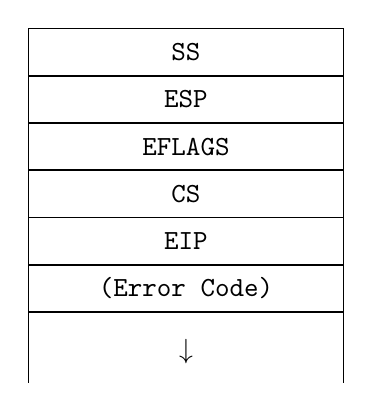
\begin{tikzpicture}

	\node[draw, semithick, minimum width=4cm, minimum height=0.6cm] (ss)         at (0, 3.3) {\texttt{SS}};
	\node[draw, semithick, minimum width=4cm, minimum height=0.6cm] (esp)        at (0, 2.7) {\texttt{ESP}};
	\node[draw, semithick, minimum width=4cm, minimum height=0.6cm] (eflags)     at (0, 2.1) {\texttt{EFLAGS}};
	\node[draw, semithick, minimum width=4cm, minimum height=0.6cm] (cs)         at (0, 1.5) {\texttt{CS}};
	\node[draw, semithick, minimum width=4cm, minimum height=0.6cm] (eip)        at (0, 0.9) {\texttt{EIP}};
	\node[draw, semithick, minimum width=4cm, minimum height=0.6cm] (error_code) at (0, 0.3) {\texttt{(Error Code)}};
	\node[                                    minimum height=0.6cm]              at (0,-0.5) {$\downarrow$};

	\draw[semithick] (-2, 0) -- (-2, -0.9);
	\draw[semithick] ( 2, 0) -- ( 2, -0.9);
\end{tikzpicture}

			\caption{État de la pile noyau après qu'une faute (ou une interruption) soit survenue en espace utilisateur\\Reproduction partielle du manuel Intel \cite{intel_interrupt_stack}}
			\label{fig:proc_interrupt_stack}
		\end{figure}

		Pour unifier la structure des données sur la pile du noyau entre toutes les fautes et interruptions, le bout d'assembleur s'exécutant en sortie de faute va pousser une valeur de bourrage sur la pile si le processeur n'a pas poussé de code d'erreur. Il va pousser le niveau d'interruption de la faute sur la pile à des fins informatives. La routine assembleur va poursuivre en complétant le contexte d'exécution qui avait été partiellement sauvé par le processeur en poussant les registres généraux sur la pile. Ceci complète la structure \texttt{int\_ctx\_t} représentant le contexte d'exécution de la partition fautive. Enfin, le bout d'assembleur va pousser un pointeur vers cette structure. Cette routine assembleur s'achève en appelant le code C qui sera chargé de récupérer les arguments pour appeler le bloc de code \texttt{getParentPartDescCont}.

		\begin{figure}[!ht]
			\centering
\begin{tikzpicture}

	\node[draw, semithick, minimum width=4cm, minimum height=0.6cm] (ss)         at (0, 3.3) {\texttt{SS}};
	\node[draw, semithick, minimum width=4cm, minimum height=0.6cm] (esp)        at (0, 2.7) {\texttt{ESP}};
	\node[draw, semithick, minimum width=4cm, minimum height=0.6cm] (eflags)     at (0, 2.1) {\texttt{EFLAGS}};
	\node[draw, semithick, minimum width=4cm, minimum height=0.6cm] (cs)         at (0, 1.5) {\texttt{CS}};
	\node[draw, semithick, minimum width=4cm, minimum height=0.6cm] (eip)        at (0, 0.9) {\texttt{EIP}};
	\node[draw, semithick, minimum width=4cm, minimum height=0.6cm] (error_code) at (0, 0.3) {\texttt{(Error Code)}};
	\node[draw, semithick, minimum width=4cm, minimum height=0.6cm] (int_level)  at (0,-0.3) {\texttt{Interrupt Level}};
	\node[draw, semithick, minimum width=4cm, minimum height=1.8cm, align=center] (greg) at (0,-1.5) {Registres généraux\\\texttt{(8 dwords)}};
	\node[draw, semithick, minimum width=4cm, minimum height=0.6cm] (ctx_ptr)    at (0,-2.7) {\texttt{int\_ctx\_t *}};
	\node[                                    minimum height=0.6cm]              at (0,-3.5) {$\downarrow$};

	\draw[semithick] (-2, -3) -- (-2, -3.9);
	\draw[semithick] ( 2, -3) -- ( 2, -3.9);

	\node[left=0.5cm of eflags, minimum width=3cm] (iret_ctx_t) {\texttt{iret\_ctx\_t}};
	\draw[dashed, thin] (ss.north west) -- (iret_ctx_t.north |- ss.north west) -- (iret_ctx_t.north);
	\draw[dashed, thin] (eip.south west) -- (iret_ctx_t.south |- eip.south west) -- (iret_ctx_t.south);

	\node[left=0.5cm of greg,   minimum width=3cm] (pushad_regs_t) {\texttt{pushad\_regs\_t}};
	\draw[dashed, thin] (pushad_regs_t.north) -- (pushad_regs_t.north |- greg.north west) -- (greg.north west);
	\draw[dashed, thin] (pushad_regs_t.south) -- (pushad_regs_t.south |- greg.south west) -- (greg.south west);

	\node[right=0.5cm of eip.south east, minimum width=3cm] (int_ctx_t) {\texttt{int\_ctx\_t}};
	\draw[dashed, thin] (ss.north east) -- (int_ctx_t.north |- ss.north east) -- (int_ctx_t.north);
	\draw[dashed, thin] (greg.south east) -- (int_ctx_t.south |- greg.south east) -- (int_ctx_t.south);

	\draw[dashed, thin] (ctx_ptr.east) -- (int_ctx_t.320 |- ctx_ptr.east);
	\draw[dashed, thin, ->] (int_ctx_t.320 |- ctx_ptr.east) -- (int_ctx_t.320);
\end{tikzpicture}

			\caption{État de la pile noyau après la routine assembleur complétant la structure \texttt{int\_ctx\_t}}
			\label{fig:interrupt_stack}
		\end{figure}

		Cette fonction s'appelle \texttt{faultInterruptHandler} ; son prototype est donné dans le listing \ref{code:faultInterruptHandler_proto}. Son code est trop long pour être inclus dans ce chapitre mais vous pouvez le retrouver en annexe \ref{code:faultInterruptHandler}.

		\begin{listing}[!ht]
			\ccode{code/faultInterruptHandler_proto.c}
			\caption{Prototype de la fonction calculant les arguments du service lors d'une faute}
			\label{code:faultInterruptHandler_proto}
		\end{listing}

		Tout comme l'appel du service par la \emph{callgate}, la fonction \texttt{faultInterruptHandler} commence par créer un nouveau contexte générique de type \texttt{user\_ctx\_t} à partir du contexte fautif précédemment créé. Ceci permet d'avoir la même représentation du contexte entre les différents points d'entrée du service, comme évoqué dans la section \ref{sec:context_harmonisation}. Cependant, le niveau de faute sera utilisé par la fonction comme argument \texttt{targetInterrupt}, pour que le parent soit reveillé avec le contexte lié à la faute.
		La fonction récupère ensuite le descripteur de partition fautive grâce à la variable globale de Pip indiquant la partition s'exécutant en espace utilisateur, qui deviendra l'argument \texttt{sourcePartDesc}. Elle récupère aussi l'état de ses drapeaux, liés aux arguments \texttt{flagsOnYield} et \texttt{flagsOnWake}. La fonction va décider où sauvegarder le contexte de la partition fautive en fonction de ces drapeaux. L'implémentation actuelle considère que si le mot mémoire représentant les drapeaux est égal à zéro, la partition ne souhaitait pas être interrompue (on parle de \emph{Virtual CLI}, en référence à l'instruction assembleur désactivant les interruptions). L'état sera alors sauvegardé dans l'espace mémoire pointé à l'index \texttt{CLI\_SAVE\_INDEX}. Si les drapeaux sont différents de zéro, alors l'autre indice réservé, \texttt{STI\_SAVE\_INDEX} sera utilisé pour l'argument \texttt{sourceContextSaveIndex}.
		Enfin, la fonction récupère le \emph{Page Directory} de la partition à partir de son descripteur qui servira d'argument \texttt{sourcePageDir}.

		Lorsque tous les arguments ont été récupérés\footnote{l'argument \texttt{nbL} de l'appel a été omis du texte principal car il est peu intéressant. Cet argument est en fait un paramètre de l'implémentation précisant le nombre d'indirections dans les structures de configurations de la MMU, soit 2 dans l'implémentation Intel x86}, la fonction est prête à appeler le bloc de code \texttt{getParentPartDescCont}.

		\paragraph{Cas des doubles fautes} Il est possible que l'appel au service échoue lors des vérifications pour le transfert de flôt d'exécution. Lorsque ce transfert est dû à une faute, la partition l'ayant déclenchée n'est plus en mesure de recevoir le flôt d'exécution : elle déclencherait à nouveau la faute. Ainsi, il faut que le service propose une voie de transfert de flôt d'exécution dont le succès ne dépend que de la bonne configuration de la partition ayant la responsabilité de la partition fautive -- c'est à dire son parent, la partition recevant le flot d'exécution.
		Dans le cas où le parent ne serait pas non plus en mesure de recevoir le flôt d'exécution, le flôt d'exécution serait redirigé vers le parent de la partition parent et remonterai la chaîne de responsabilité, jusqu'à ce qu'une partition reçoive le flôt d'exécution sans erreur, ou jusqu'à ce que la partition racine elle même échoue à le recevoir.

		C'est pourquoi la fonction récupérant les arguments appelle à son tour une autre fonction appelée \texttt{propagateFault} (cette fonction est disponible en annexe, voir listing \ref{code:faultInterruptHandler}). Cette fonction est chargée de faire l'appel au bloc de code \texttt{getParentPartDescCont} et de gérer les éventuelles erreurs pouvant survenir après un appel à ce bloc. 
		Les différentes étapes logicielles permettant d'utiliser le service pour une faute sont résumés dans la figure \ref{fig:fault_software}. Il y a trois cas d'erreurs distincts gérés par la fonction :
		\begin{itemize}
			\item le cas où la fonction ayant réalisé la faute est la partition racine : dans ce cas là, il n'y a plus rien à rattraper, la partition racine étant la base de confiance absolue du système -- si elle échoue le système s'écroule. Le service s'arrête alors sur une boucle infinie.
			\item le cas où le service n'a pas réussi à récupérer la VIDT de la partition fautive, ou l'espace mémoire permettant de sauvegarder le contexte : dans ce cas, la sauvegarde du contexte de la partition fautive est omise, et l'exécution reprend au bloc de code \texttt{getTargetVidtCont}.
			\item dans tous les autres cas d'erreur, la partition parent n'est pas correctement configurée et n'est pas en mesure de rattraper la faute. Dans ce cas, la fonction \texttt{propagateFault} fait un appel récursif. La faute est redirigée sur le parent de la cible actuelle, et le niveau d'interruption de la faute est changé au niveau correspondant à la double faute.
		\end{itemize}


		\begin{figure}[!ht]
			\centering
			\begin{tikzpicture}[>=triangle 45,font=\sffamily, every text node part/.style={align=center}, scale=1, every node/.style={transform shape}] {

	\node[draw, fill=white, ultra thin, drop shadow, minimum height=1cm] (assembly) at (9,5.5) {Complétion du contexte d'exécution};
	\node[draw, fill=white, ultra thin, drop shadow, minimum height=1cm] (args) at (7.5,4.25) {Récupération des arguments};
	\node[draw, fill=white, ultra thin, drop shadow, minimum height=1.5cm, align=center] (call) at (6,2.75) {Appel au service\\Gestion des erreurs};
	\node[draw, fill=white, ultra thin, drop shadow, minimum height=1cm] (parents_checks) at (0.5,2.75) {Récupération partition parent};
	\node[draw, fill=white, ultra thin, drop shadow, minimum height=1cm] (callee_vidt) at (0.5,1) {Récupération VIDT appelé};

	\node[draw, fill=white, ultra thin, drop shadow={shadow xshift=0.07cm,shadow yshift=-0.07cm}, minimum height=1cm, circle] (guru_meditation) at (10.5,1.5) {$\infty$};

	\node[above=0.2cm of assembly, fill=red!30, drop shadow={shadow xshift=0.05cm,shadow yshift=-0.05cm}] (interruptgate) {\small{\texttt{Faute - Interrupt gate}}};

	\draw[->] (assembly.345) to[in=0, out=270] (args);
	\draw[->] (args.340) to[in=0, out=270] (call);

	\draw[->] (call.173) to[in=0, out=180] (parents_checks.5);
	\draw[->, dashed, gray] (parents_checks.355) to[in=180, out=0] (call.187);
	\draw[->, dashed, gray] (call.220) to[in=0, out=270] (callee_vidt);
	\draw[->, dashed, gray] (call.260) to[in=240, out=280] (call.330);
	\draw[->, dashed, gray] (call) -- (guru_meditation);

	\node (separation) at (3.625,6) {};
	\draw[semithick, dotted] (separation) -- (3.625, 0.5);
	\node[below left=0.4cm of separation, fill=gray!30, drop shadow={shadow xshift=0.05cm,shadow yshift=-0.05cm}] (service) {\small{\texttt{Blocs du service}}};
}

\end{tikzpicture}

			\caption{Résumé des différents blocs logiciels permettant d'appeler le service après une faute}
			\label{fig:fault_software}
		\end{figure}

		\subsubsection{Implémentation des interruptions utilisant le service sur l'architecture x86}

		La même méthode a été employée pour gérer les interruptions matérielles avec le service. Pour rappel, les interruptions matérielles doivent arriver à la partition racine. Il n'y a pas de bloc de code récupérant la partition racine directement, il faut donc commencer à exécuter le service après les blocs de code récupérant le descripteur de partition. Ceci permet d'injecter dans les paramètres le descripteur de la partition racine à la place des partitions initialement prévues par les blocs précédents.

		Le bloc idéal pour devoir récupérer le moins d'arguments possibles est le bloc \texttt{getSourceVidtCont}. Le prototype du bloc est présenté en listing \ref{code:getSourceVidtCont_proto}.

		\begin{listing}[!ht]
			\coqcode{code/getSourceVidtCont.v}
			\caption{Prototype du bloc de code \texttt{getSourceVidtCont}, ciblé par les interruptions matérielles.}
			\label{code:getSourceVidtCont_proto}
		\end{listing}

		Le cheminement jusqu'à l'exécution du bloc du service est extrêmement similaire à celui concernant les fautes. De la même manière que pour une faute, lorsqu'une interruption matérielle arrive, le processeur va récupérer l'\emph{interrupt gate} correspondante dans l'\emph{IDT} (pour rappel, les niveaux d'interruptions correspondants aux interruptions matérielles vont de 32 à 47). Cette similitude continue jusqu'à la récupération des arguments : le processeur change de pile et pousse les mêmes éléments que ceux présentés précédemment en figure \ref{fig:interrupt_stack}, puis une routine assembleur complète le contexte d'exécution de type \texttt{int\_ctx\_t}, et appelle finalement la fonction de récupération des arguments \texttt{hardwareInterrupthandler}. Les arguments à récupérer par la fonction sont les mêmes que pour le bloc \texttt{getParentPartDescCont} et sont récupérés de la même manière, mis à part l'argument \texttt{targetPartDesc}. Cet argument est l'adresse réelle du descripteur de la partition recevant le flôt d'exécution, qui devra donc être le descripteur de la partition racine. La fonction récupère ce descripteur au travers d'une variable globale de Pip.

		L'appel du bloc de code \texttt{getSourceVidtCont} peut aussi se solder par une erreur : si l'origine de cette erreur est le fait que la VIDT de la partition n'est pas accessible ou que l'emplacement de sauvegarde de son contexte n'est pas accessible, alors la sauvegarde de contexte est omise et la fonction appelle le bloc de code \texttt{getTargetVidtCont}. Une autre erreur indiquerait que la partition racine n'est pas en mesure de récupérer le flôt d'exécution ; dans ce cas la fonction arrête l'exécution en rentrant dans une boucle infinie.

		\begin{figure}[!ht]
			\centering
			\begin{tikzpicture}[>=triangle 45,font=\sffamily, every text node part/.style={align=center}, scale=1, every node/.style={transform shape}] {

	\node[draw, fill=white, ultra thin, drop shadow, minimum height=1cm] (assembly) at (9,5.5) {Complétion du contexte d'exécution};
	\node[draw, fill=white, ultra thin, drop shadow, minimum height=1cm] (args) at (7.5,4.25) {Récupération des arguments};
	\node[draw, fill=white, ultra thin, drop shadow, minimum height=1.5cm, align=center] (call) at (6,2.75) {Appel au service\\Gestion des erreurs};
	\node[draw, fill=white, ultra thin, drop shadow, minimum height=1cm] (parents_checks) at (0.5,2.75) {Récupération VIDT appelant};
	\node[draw, fill=white, ultra thin, drop shadow, minimum height=1cm] (callee_vidt) at (0.5,1) {Récupération VIDT appelé};

	\node[draw, fill=white, ultra thin, drop shadow={shadow xshift=0.07cm,shadow yshift=-0.07cm}, minimum height=1cm, circle] (guru_meditation) at (10.5,1.5) {$\infty$};

	\node[above=0.2cm of assembly, fill=red!30, drop shadow={shadow xshift=0.05cm,shadow yshift=-0.05cm}] (interruptgate) {\small{\texttt{Interruption matérielle - Interrupt gate}}};

	\draw[->] (assembly.345) to[in=0, out=270] (args);
	\draw[->] (args.340) to[in=0, out=270] (call);

	\draw[->] (call.173) to[in=0, out=180] (parents_checks.5);
	\draw[->, dashed, gray] (parents_checks.355) to[in=180, out=0] (call.187);
	\draw[->, dashed, gray] (call.220) to[in=0, out=270] (callee_vidt);
	\draw[->, dashed, gray] (call) -- (guru_meditation);

	\node (separation) at (3.625,6) {};
	\draw[semithick, dotted] (separation) -- (3.625, 0.5);
	\node[below left=0.4cm of separation, fill=gray!30, drop shadow={shadow xshift=0.05cm,shadow yshift=-0.05cm}] (service) {\small{\texttt{Blocs du service}}};
}

\end{tikzpicture}

			\caption{Résumé des différents blocs logiciels permettant d'appeler le service après une interruption matérielle}
			\label{fig:interrupt_software}
		\end{figure}

		À l'exception de l'état des piles lors des différents transferts de flôt d'exécution, le fonctionnement du service et des routines permettant d'y accéder restent rigoureusement les même entre toutes les architectures. 
		\newpage

		\begin{figure}[!ht]
			\begin{tikzpicture}[>=triangle 45,font=\sffamily, every text node part/.style={align=center}, scale=1, every node/.style={transform shape}] {
	\node[draw, fill=white, ultra thin, drop shadow, minimum width=3cm, minimum height=1cm] (int_no_checks) at (0,9.5) {\footnotesize{Vérification du n° contexte appelé}};
	\node[draw, fill=white, ultra thin, drop shadow, minimum width=3cm, minimum height=1cm] (ctx_sav_checks) at (0,8.45) {\footnotesize{Vérification du n° de sauvegarde du contexte}};
	\node[draw, fill=white, ultra thin, drop shadow, minimum width=3cm, minimum height=1cm] (child_checks) at (-3, 6.95) {\footnotesize{Récupération partition enfant}};
	\node[draw, fill=white, ultra thin, drop shadow, minimum width=3cm, minimum height=1cm] (parent_checks) at (3, 6.95) {\footnotesize{Récupération partition parent}};
	\node[draw, fill=white, ultra thin, drop shadow, minimum width=3cm, minimum height=1cm] (source_checks) at (0, 5.45) {\footnotesize{Récupération VIDT appelant}};
	\node[draw, fill=white, ultra thin, drop shadow, minimum width=3cm, minimum height=1cm] (target_checks) at (0, 4.40) {\footnotesize{Récupération VIDT appelé}};
	\node[draw, fill=white, ultra thin, drop shadow, minimum width=3cm, minimum height=1cm] (target_ctx) at (0, 3.35) {\footnotesize{Récupération contexte appelé}};
	\node[draw, fill=white, ultra thin, drop shadow, minimum width=3cm, minimum height=1.5cm] (save_ctx) at (-3, 1.60) {\footnotesize{Vérification de l'espace de sauvegarde du contexte}\\\footnotesize{Sauvegarde du contexte}};
	\node[draw, fill=white, ultra thin, drop shadow, minimum width=3cm, minimum height=2cm] (switch_ctx) at (2, -0.65) {\footnotesize{Changement d'espace d'adressage}\\\footnotesize{Mise à jour des structures internes de Pip}\\\footnotesize{Chargement du contexte appelé}};
	\draw[->] (ctx_sav_checks) to[in=90, out=200] (child_checks.20);\draw[->] (ctx_sav_checks) to[in=90, out=340] (parent_checks.160);
	\draw[->] (child_checks) to[in=90, out=0] (source_checks.140);\draw[->] (parent_checks) to[in=90, out=180] (source_checks.40);
	\draw[->] (target_ctx) to[in=90, out=180] (save_ctx);\draw[->] (target_ctx) to[in=90, out=340] (switch_ctx);
	\draw[->] (save_ctx) to[in=180, out=270] (switch_ctx);

	%\node[above right=0.2cm of parent_checks.60, fill=red!30, drop shadow={shadow xshift=0.05cm,shadow yshift=-0.05cm}] (fault) {\small{\texttt{Entrée fautes}}};
	\node[right=0.2cm of parent_checks.07, fill=red!30, drop shadow={shadow xshift=0.05cm,shadow yshift=-0.05cm}] (fault) {\small{\texttt{Entrée fautes}}};
	\node[above right=0.2cm of parent_checks.45, fill=red!30, drop shadow={shadow xshift=0.05cm,shadow yshift=-0.05cm}] {\small{\texttt{Entrée int. logicielle}}};
	\node[right=0.2cm of target_checks.07, fill=red!30, drop shadow={shadow xshift=0.05cm,shadow yshift=-0.05cm}]{\small{\texttt{Entrée double fautes}}};
	\node[above=0.2cm of int_no_checks.90, fill=red!30, drop shadow={shadow xshift=0.05cm,shadow yshift=-0.05cm}]{\small{\texttt{Entrée explicite}}};
	\node[left=0.2cm of source_checks.173, fill=red!30, drop shadow={shadow xshift=0.05cm,shadow yshift=-0.05cm}]{\small{\texttt{Entrée int. matérielle}}};
}

\end{tikzpicture}

			\caption{Vue éclatée des blocs constituant le service}
			\label{fig:callgraph}
		\end{figure}
		\newpage
	\section{Preuve d'isolation}

		Cette section a pour but de décrire le processus d'établissement de la preuve d'isolation de Pip sur le service. La première sous-section décrira tout d'abord les nouvelles fonctions introduites dans l'interface de la monade d'état ainsi que la raison de leur inclusion. Ces fonctions sont accompagnées de nouveaux types, qui seront aussi explicités. La seconde sous-section fera un rappel des propriétés d'isolation de Pip. La dernière sous-section décrira le processus d'établissement de la preuve.\\

		\textbf{Note importante :} Dans un soucis de transparence et d'intégrité scientifique, je souhaite préciser que la preuve d'isolation reposant sur les modèles présentés dans cette section n'est pas encore complète. En effet, nous avons récemment repéré une simplification abusive dans le modèle de la fonction \texttt{writeContext}. Cette trouvaille a mené à la réécriture du modèle de la fonction et a rendu caduque la preuve d'isolation précédemment établie sur l'ancien modèle. Dans cette section, nous présenterons néanmoins le nouveau modèle qui reflète le comportement attendu de la fonction, et qui est plus intéressant. Ce nouveau modèle ne change en rien l'implémentation réelle de cette fonction : ces changements sont cantonnés au monde des mathématiques. De plus, ce nouveau modèle n'introduit pas d'obstacle particulier à l'établissement de la preuve d'isolation. Elle n'a pas été établie par manque de temps entre sa découverte et l'écriture de ce document. Nous reviendrons cependant sur cette erreur de modélisation dans la section suivante, qui révèle la subtilité de l'établissement de preuves au travers de modèles.

		\subsection{Définition de l'interface avec la monade}

		Cette sous-section est dédiée à la définition des nouveaux éléments de l'interface avec la monade. Nous discuterons d'abord des nouveaux types et de ce qu'ils représentent, puis nous discuterons des fonctions.

		\subsubsection{Nouveaux types intégrés à la monade}

		\paragraph{\texttt{userValue}} Le type \texttt{userValue} est un type \emph{opaque}, c'est à dire un type dont les valeurs n'ont pas vocation à être manipulées dans le modèle. Le type \texttt{userValue} indique une valeur arbitraire provenant de l'espace utilisateur. Cette valeur doit subir des tests avant de pouvoir être transformée en un type sain et utilisable par le noyau. Prenons par exemple le type \texttt{index}. \texttt{index} est un entier naturel dont la valeur ne peut dépasser le nombre de mots mémoire dans une page. Afin de s'assurer qu'un indice passé en paramètre par l'utilisateur respecte bien ces contraintes, le service va le traiter comme une \texttt{userValue}. Le service vérifie alors que la contrainte est bien respectée, puis raffine le type de la valeur en un \texttt{index}. Pour certains types de valeurs, il n'est pas nécessaire d'utiliser le type \texttt{userValue}. Ceci est vrai pour les types dont l'intégralité des valeurs représentables sont des valeurs valides, comme par exemple les adresses virtuelles.

		Le type \texttt{userValue} étant un type opaque, son modèle importe peu. Il est représenté par un \texttt{nat}.

		\paragraph{\texttt{interruptMask}} Le type \texttt{interruptMask} est un type \emph{opaque} représentant les drapeaux servant aux partitions à indiquer si elles souhaitent être interrompues ou non. Ce type est entouré d'une interface permettant de récupérer ces drapeaux depuis un contexte d'exécution, d'appliquer ces drapeaux à une partition, de sauver ces drapeaux dans un contexte d'exécution, ainsi que d'interprêter ces drapeaux. La mise en place d'un tel mécanisme est fortement lié à la plateforme et a été laissée libre à l'implémentation. Le type est representé comme une liste de booléens dont la longueur est égale au nombre de niveaux d'interruptions, cependant cette information n'est jamais exploitée dans le modèle.
		\begin{listing}[!ht]
			\begin{minted}{coq}
Record interruptMask := {
    m  :> list bool;
    Hm :  length m = maxVint+1;
}.
			\end{minted}
			\caption{Représentation du type \texttt{interruptMask} dans le modèle}
		\end{listing}

		\paragraph{\texttt{contextAddr}} Le type \texttt{contextAddr} est un type \emph{opaque} représentant l'adresse d'un contexte d'exécution. Il est muni de deux fonctions : une permettant d'écrire ce contexte à une adresse donnée, l'autre l'applicant au système qui reprendra le flôt d'exécution lié. Le type est représenté par un \texttt{nat}.


		\subsubsection{Nouvelles fonctions de l'interface}

		Certaines de ces nouvelles fonctions font partie de l'interface des nouveaux types présentés dans les paragraphes précédent. Tout d'abord le type \texttt{userValue} a engendré deux nouvelles fonctions :
		\paragraph{\mintinline{c}{bool checkIndexPropertyLTB(userValue userIndex);}}~\\
		Cette fonction retourne vrai si la valeur passée en paramètre respecte la contrainte du type \texttt{index} ; la valeur doit être inférieure au nombre de mots mémoire dans une page. Voici son modèle :

		\begin{listing}[!ht]
			\begin{minted}{coq}
Definition checkIndexPropertyLTB (userIndex : userValue) : LLI bool :=
ret (Nat.ltb userIndex tableSize).
			\end{minted}
			\caption{Modèle de la fonction \texttt{checkIndexPropertyLTB}}
		\end{listing}
		Cette fonction de l'interface a cependant été maladroitement choisie, car le choix de la valeur de la comparaison \texttt{tableSize} relève de la responsabilité de l'implémentation, alors qu'elle aurait pu rester dans le code du service. La fonction pertinente à ajouter dans l'interface au lieu de celle-ci aurait dû être la fonction de comparaison entre une \texttt{userValue} et un \texttt{index}.

		\paragraph{\mintinline{c}{index userValueToIndex(userValue userIndex);}}~\\
		Cette fonction transforme la valeur de type \texttt{userValue} en fonction de type \texttt{index}. Cette fonction n'a pas d'effet particulier sur la valeur.
		Son modèle est disponible en listing \ref{code:userValueToIndex}. Ce modèle met en lumière que la valeur \texttt{userIndex} doit être inférieure à la constante \texttt{tableSize}, qu'une preuve en soit établie, et que cette preuve soit passée au constructeur du type \texttt{index} (ici déterminée automatiquement par Coq au travers du symbole \texttt{\_}).
		\begin{listing}[!ht]
			\begin{minted}{coq}
Program Definition userValueToIndex (userIndex : userValue) : LLI index :=
    if lt_dec userIndex tableSize
    then
        ret (Build_index userIndex _ )
    else undefined 85.
			\end{minted}
			\caption{Modèle de la fonction \texttt{userValueToIndex}}
			\label{code:userValueToIndex}
		\end{listing}

		\newpage
		Le service a ajouté quatre fonctions dans l'interface qui intéragissent avec le type \texttt{interruptMask}.

		\mintinline{c}{interruptMask getInterruptMaskFromCtx(contextAddr context)} est la première fonction permettant de récupérer les drapeaux présents dans un contexte d'exécution. La seconde fonction~ \mintinline{c}{bool noInterruptRequest(interruptMask flagsOnWake)} permet d'interpréter les drapeaux passés en paramètres pour renvoyer si la partition ne souhaite pas être interrompue. La troisième fonction en rapport avec le type \texttt{interruptMask} est la fonction \mintinline{c}{void setInterruptMask(uint32_t interrupt_state)} qui permet d'appliquer les masques à la partition courante. La dernière fonction ajoutée,~~\mintinline{c}{uint32_t}\\ \mintinline{c}{get_self_int_state()}, permet de récupérer les drapeaux de la partition courante.

		Du point de vue du modèle, ces fonctions sont peu intéressantes. Elles n'ont pas été intégrées car la position des drapeaux n'a pas été définie dans l'interface et peut donc être placée arbitrairement par l'implémentation. L'implémentation Intel x86, place ces drapeaux dans le descripteur de la partition, afin que leur écriture soit atomique. Ainsi, ces fonctions renvoient soit une valeur arbitraire, soit n'ont aucun effet sur le modèle. La fonction \mintinline{c}{uint32_t get_self_int_state()} n'a pas été modélisée car elle n'apparait pas dans le service, mais dans les fonctions de récupération des arguments discutés en section \ref{sec:service_generalisation}.\\

%		\paragraph{\mintinline{c}{interruptMask getInterruptMaskFromCtx(contextAddr context);}}
%			Cette fonction récupère les drapeaux enregistrés dans un contexte d'exécution. Son modèle retourne des drapeaux arbitraires.
%			\begin{listing}[!ht]
%				\begin{minted}{coq}
%Definition getInterruptMaskFromCtx (context : contextAddr) :
%LLI interruptMask := ret int_mask_d.
%				\end{minted}
%				\caption{Modèle de la fonction \texttt{getInterruptMaskFromCtx}}
%				\label{code:getInterruptMaskFromCtx}
%			\end{listing}
%
%		\paragraph{\mintinline{c}{bool noInterruptRequest(interruptMask flagsOnWake);}}
%			Cette fonction renvoie vrai si les drapeaux passés en paramètres indiquent que la partition ne souhaite pas se faire interrompre. Le modèle de cette fonction renvoie une valeur arbitraire.
%			\begin{listing}[!ht]
%				\begin{minted}{coq}
%Definition noInterruptRequest (flags : interruptMask) : LLI bool :=
%    ret true.
%				\end{minted}
%				\caption{Modèle de la fonction \texttt{noInterruptRequest}}
%				\label{code:noInterruptRequest}
%			\end{listing}
%
%		\paragraph{\mintinline{c}{void setInterruptMask(uint32_t interrupt_state);}}
%			Cette fonction applique les drapeaux à la partition courante. Cette fonction n'a aucun effet dans le modèle.
%			\begin{listing}[!ht]
%				\begin{minted}{coq}
%Definition setInterruptMask (mask : interruptMask) : LLI unit :=
%    ret tt.
%				\end{minted}
%				\caption{Modèle de la fonction \texttt{setInterruptRequest}}
%				\label{code:setInterruptRequest}
%			\end{listing}
%
%		\paragraph{\mintinline{c}{uint32_t get_self_int_state();}}
%			Cette fonction permet de récupérer les drapeaux de la partition courante. Cette fonction n'a pas de modèle car elle n'est utilisée que dans les routines de récupération des arguments pour le transfert de flôt d'exécution lors de fautes ou d'interruptions.

		Les fonctions les plus intéressantes de cet ajout à l'interface sont celles qui manipulent le type \texttt{contextAddr}.

		\paragraph{\mintinline{c}{contextAddr vaddrToContextAddr(vaddr contextVAddr);}}~\\
		Cette fonction convertit une adresse virtuelle en pointeur vers un contexte d'exécution. Le modèle de cette fonction renvoie une valeur arbitraire.

		\paragraph{\mintinline{c}{void loadContext(contextAddr ctx, bool enforce_interrupts);}}~\\
		Cette fonction charge le contexte d'exécution pointé par \texttt{ctx}, en s'assurant que le futur flôt d'exécution sera interruptible si \texttt{enforce\_interrupts} est vrai.

		Cette fonction est intéressante car elle ne peut être écrite en Gallina, le langage de Coq. En effet, Coq s'assure que tous les programmes écrits en Gallina terminent, ce qui n'est pas le cas de cette fonction. Par exemple, dans l'implémentation Intel x86, cette fonction charge tout les registres généraux puis pousse une petite partie du contexte sur pile, et exécute l'instruction assembleur \texttt{iret}. À partir du moment où cette instruction a été exécutée, le flôt d'exécution a déjà changé : la pile et le pointeur d'instruction ne sont plus les mêmes. De ce fait cette fonction n'a aucun effet dans le modèle.

		\begin{listing}[!ht]
			\begin{minted}{coq}
Definition loadContext (contextToLoad : contextAddr)
                       (enforce_interrupt : bool) : LLI unit :=
    ret tt.
			\end{minted}
			\caption{Modèle de la fonction \texttt{loadContext}}
			\label{code:loadContext}
		\end{listing}

		Cependant, il n'est pas \emph{nécessaire} que cette fonction ne retourne pas. En effet, dans l'implémentation actuelle sur Intel x86, la fonction copie le contexte sur le dessus de la pile et le charge immédiatement. Il s'avère que ce code de chargement est aussi disponible dans les portions d'assembleur appelant le service, dans le cas où une erreur surviendrait pendant l'exécution du service. Dans ce cas, le service retourne prématurément pour signaler une erreur et la fonction \texttt{loadContext} n'est jamais atteinte. Ces portions de code restaurent le contexte appelant le service, mais il serait possible que la fonction \texttt{loadContext} vienne modifier ce contexte initial pour qu'il corresponde au nouveau contexte à charger. Ainsi, le transfert de flot d'exécution ne s'opérerait pas dans la fonction \texttt{loadContext}, mais dans la portion d'assembleur de retour au contexte initial. Ainsi, il serait possible d'éviter cette dualité entre le monde du modèle qui retourne et renvoie un succès, et le monde réel qui ne retourne pas et charge directement le contexte dans la fonction. Cette approche est néanmoins beaucoup plus compliquée à mettre en place comparée à une simple copie des données sur le sommet de la pile, et n'apporte pour le moment pas d'autre avantage que l'agréable sentiment d'harmonie dans la création.

		\paragraph{\mintinline{c}{void writeContext(contextAddr ctx, vaddr ctxSaveVAddr, interruptMask}}~~\\
		   \textbf{\mintinline{c}{flagsOnWake);}}~\\
			Cette fonction écrit le contexte d'exécution pointé par \texttt{ctx} à l'adresse virtuelle \texttt{ctxSaveVAddr}, en y écrivant les drapeaux \texttt{flagsOnWake}. Cette fonction est différente des autres fonctions d'écriture de l'interface avec la monade car elle effectue plusieurs écritures successives en mémoire. De plus, ces écritures sont faites en espace utilisateur. Son modèle se contente d'appeler une fonction récursive qui va itérer sur la taille d'un contexte, et écrire aux adresses virtuelles successives une valeur arbitraire.\\

		\begin{listing}[!ht]
			\begin{minted}{coq}
Definition writeContext (callingContextAddr : contextAddr)
                        (contextSaveAddr : vaddr)
                        (flagsOnWake : interruptMask) : LLI unit :=
    perform maxIdx := getMaxIndex in
    perform idxContextInPage := ret (List.last contextSaveAddr index_d) in
    writeContextAux contextSaveAddr idxContextInPage maxIdx contextSize.

Fixpoint writeContextAux (contextSaveAddr : vaddr) (currIdx : index)
                         (maxIdx : index) (bound : nat) : LLI unit :=
  match bound with
  | 0 => ret tt
  | S dec_bound =>
    storeVirtual contextSaveAddr currIdx vaddrDefault ;;
    if idxEq currIdx maxIdx then
      writeContextAux (getNextVaddr contextSaveAddr) idx0 maxIdx dec_bound
    else
      perform nextIdx := idxSuccM currIdx in
      writeContextAux (getNextVaddr contextSaveAddr) nextIdx maxIdx dec_bound
  end.
			\end{minted}
			\caption{Modèle de la fonction \texttt{writeContext} et sa fonction auxiliaire récursive}
			\label{code:writeContextModel}
		\end{listing}

		Les écritures multiples de la fonction \texttt{writeContext} ont mené à des vérifications supplémentaires qui ont nécessité l'ajout de deux fonctions dans l'interface. La première est \mintinline{c}{vaddr getNthVAddrFrom(vaddr base, uint32_t size)}. Cette fonction retourne l'adresse virtuelle se trouvant à l'adresse de base plus une certain nombre d'octets \texttt{size}. Cette fonction permet notamment de récupérer la dernière adresse d'un contexte d'exécution, afin de vérifier qu'elle est bien valide avant d'entamer l'écriture.\\
		La seconde est \mintinline{c}{bool firstVAddrGreaterThanSecond(vaddr vaddr1, vaddr vaddr2)}, qui retourne si une adresse virtuelle est plus grande que la seconde. Cela permet au service de vérifier qu'un overflow n'a pas eu lieu lors du calcul de la dernière adresse du contexte.

		La fonction \mintinline{c}{vaddr getVaddrVIDT()} fait aussi partie des nouveaux ajouts à l'interface, et retourne l'adresse fixe de la VIDT. Cette valeur est définie comme la dernière page de l'espace d'adressage virtuel.

		Enfin, la fonction \mintinline{c}{void updateMMURoot(page MMURoot)} a été ajoutée. Cette fonction applique un nouvel espace d'adressage décrit par \texttt{MMURoot}. Dans l'implémentation Intel, cette fonctionne écrit le Page Descriptor \texttt{MMURoot} -- structure racine de la configuration de la MMU -- dans le registre \texttt{CR3} du processeur. Cette fonction est spéciale car elle aurait pu être cachée dans l'implémentation, et n'a aucun sens dans le modèle d'isolation de Pip. Elle été ajoutée dans l'optique de produire une preuve fonctionnelle du service.

		C'est sur ces différents modèles de fonction que la preuve d'isolation sera établie. Dans la prochaine section nous préciserons les propriétés d'isolation, avant de procéder à l'explication de l'établissement de la preuve.

		\subsection{Rappel des propriétes d'isolation de Pip}

		Comme exprimé dans la section \ref{sec:pip}, la preuve d'isolation de Pip repose sur trois propriétés fondamentales : la propriété d'\emph{isolation horizontale}, la propriété d'\emph{isolation noyau} ainsi que la propriété de \emph{partage verticale}. Ces trois propriétés principales sont accompagnées d'une multitude de propriétés liées à la cohérence du noyau. Certaines de ces propriétés seront mises en avant dans ce document, puisqu'elle seront discutées dans la section suivante traitant de l'établissement de la preuve du service.

			\subsubsection{Isolation horizontale}

			La propriété d'isolation horizontale stipule que deux enfants d'une même partition parent ne peuvent partager de page mémoire au travers de leur espace d'adressage ou de leurs pages de configuration. Les deux ensembles des pages concernant l'une et l'autre des partitions enfants doivent être strictement disjoints. Le listing \ref{code:horizontal_isolation} montre comment est exprimée formellement cette propriété dans l'assistant de preuve.

			\begin{listing}[!ht]
				\coqcode{code/horizontal_isolation.v}
				\caption{Propriété d'isolation horizontale telle qu'exprimée dans Coq}
				\label{code:horizontal_isolation}
			\end{listing}

			La fonction \texttt{getPartitions} récupère les pages contenant les descripteurs de partitions. La fonction \texttt{getChildren} recupère la liste des pages contenant les descripteurs de partitions de tous les enfants de la partition passée en paramètre. La fonction \texttt{getUsedPages} récupère l'ensemble des pages mémoires renseignées dans les structures de données de la partition passée en paramètre. Cela inclus les structures internes de Pip ainsi que la description de l'espace d'adressage de la partition.

			La propriété peut être lue de la sorte :
			\begin{theorem}
				Pour toutes pages de mémoire \texttt{parent}, \texttt{child1} et \texttt{child2}. Si \texttt{parent} est dans la liste des descripteurs de partitions, si \texttt{child1} et \texttt{child2} sont tous deux dans la liste des partitions enfant de \texttt{parent}, et si \texttt{child1} et \texttt{child2} sont différents, alors l'ensemble des pages utilisées par la partition \texttt{child1} est disjoint de l'ensemble des pages utilisées par la partition \texttt{child2}.
			\end{theorem}

			\subsubsection{Isolation noyau}
			\label{sec:kernel_isolation}

			La propriété d'isolation du noyau stipule que les pages de configuration d'une partition (c'est à dire les pages réquisitionnées par Pip pour y loger ses structures, notamment les structures relative à l'espace d'adressage de la partition) sont inaccessibles à \emph{n'importe quelle} partition.
			Cette propriété est exprimée formellement par le code décrit en listing \ref{code:kernel_isolation}.

			\begin{listing}[!ht]
				\coqcode{code/kernel_isolation.v}
				\caption{Propriété d'isolation du noyau telle qu'exprimée dans Coq}
				\label{code:kernel_isolation}
			\end{listing}

			La fonction \texttt{getAccessibleMappedPages} permet de récupérer les pages de mémoire renseignées comme accessibles sans privilège dans l'espace d'adressage de la partition passée en paramètre. La fonction \texttt{getConfigPages} permet de récupérer l'ensemble des pages de mémoire de la partition passée en paramètre contenant les structures internes à Pip.

			La propriété peut être lue de la sorte :
			\begin{theorem}
				Pour toutes pages de mémoire \texttt{partition1} et \texttt{partition2}. Si \texttt{partition1} et \texttt{partition2} sont toutes deux dans la liste des descripteurs de partitions, alors l'ensemble des pages contenant les structures internes de Pip relatives à la \texttt{partition2} est disjoint de l'ensemble des pages accessibles à la \texttt{partition1}.
			\end{theorem}

			\subsubsection{Partage vertical}

			La dernière propriété fondamentale d'isolation de Pip, appelée propriété de partage vertical, stipule que chaque page relative à une partition enfant fait partie de l'espace d'adressage de son parent. Ces pages concernent aussi bien les pages de configuration de la partition enfant reservées à Pip que les pages disponibles dans son espace d'adressage. Certaines pages ne sont cependant pas accessibles à la partition parent bien qu'elles soient mappées, en particulier les pages de configuration de la partition enfant réquisitionnées par Pip.

			\begin{listing}[!ht]
				\coqcode{code/vertical_sharing.v}
				\caption{Propriété de partage vertical de la mémoire telle qu'exprimée dans Coq}
				\label{code:vertical_sharing}
			\end{listing}

			La fonction \texttt{getMappedPages} permet de récupérer toutes les pages de mémoire mappées dans la partition passée en paramètre.

			La propriété peut être lue de la manière suivante :

			\begin{theorem}
				Pour toutes pages mémoire \texttt{parent} et \texttt{child}, si \texttt{parent} fait partie de la liste des descripteurs de partitions et que \texttt{child} est dans la liste des descripteurs de partitions enfant de \texttt{parent}, alors l'ensemble des pages relatives à \texttt{child} est inclus dans l'ensemble des pages mappées dans l'espace d'adressage de la partition \texttt{parent}.
			\end{theorem}

			\subsubsection{Propriétés de cohérence du noyau}

			Dans Pip, il y a 25 propriétés annexes, qui décrivent comment sont organisées les structures de données internes de Pip. Ces propriétés sont appelées les propriétés de cohérence du noyau. Ces propriétés ne seront pas détaillée ici, car seules certaines d'entre elles présentent un intérêt dans la preuve de préservation de l'isolation. Elles seront introduites au fil de l'eau dans les sections suivantes aux endroits pertinents.

		\subsection{Déroulement de la preuve d'isolation}

		Cette preuve est axée autour de deux points critiques ; la mise à jour de la partition courante, ainsi que l'écriture du contexte de la partition appelante dans son espace d'adressage. Nous commencerons par passer en revue les propriétés souhaitées ainsi que la méthode utilisée pour chacun des deux points critiques de cette preuve, puis nous verrons comment ces propriétés sont récupérées au fur et à mesure de l'exécution des blocs préliminaires du service.

			\subsubsection{Modification de la partition courante}

			Comme décrit précédemment, la modification de la partition courante s'effectue dans le bloc \texttt{switchContextCont}. La fonction responsable de cette modification est la fonction \texttt{updateCurPartition}, dont le modèle est présenté en listing \ref{code:updateCurPartition}.

			\begin{listing}[!ht]
				\coqcode{code/updateCurPartition.v}
				\caption{Modèle de la fonction \texttt{updateCurPartition} modifiant la variable contenant la partition courante}
				\label{code:updateCurPartition}
			\end{listing}

			Cette fonction est \emph{monadique}, ce qui implique qu'elle est une fonction partielle sur l'état. C'est une fonction d'écriture, elle décrit donc comment est modifié l'état lors de son exécution. Cette fonction prend en argument une page mémoire arbitraire \texttt{phyPartition} et remplace la composante \texttt{currentPartition} de l'état par le paramètre \texttt{phyPartition}. Ainsi, après l'exécution de \texttt{updateCurPartition}, si on nomme $s'$ le nouvel état produit à partir de l'état initial $s$, alors : \\

			\mintinline{coq}{s' := {| currentPartition := phyPartition ; memory := (memory s) |}}.\\

			Seules deux propriétés mentionnent directement le champ \texttt{currentPartition} de l'état : \texttt{currentPartitionInPartitionsList} et \texttt{currentPartitionIsNotDefaultPage}. Ces deux propriétés sont des propriétés de cohérence.

			\begin{listing}[!ht]
				\coqcode{code/consistencyCurPart.v}
				\caption{Propriétés de cohérence directement affectées par le changement du champ \texttt{currentPartition} de l'état}
				\label{code:consistencyCurPart}
			\end{listing}

			Ces propriétés assurent respectivement que la variable globale contenant la partition courante contiendra toujours un descripteur de partition provenant de la liste des descripteurs de partitions, et qu'elle ne soit pas égale à la valeur par défaut.

			Elles doivent être déduite de propriétés précédemment établies sur la page passée en paramètre. En particulier, on veut donc pouvoir montrer que \texttt{targetPartDesc} représente bien un descripteur de partition et qu'il n'est pas nul. Ces deux propriétés, décrites en listing \ref{code:curPartProperties}, doivent avoir été établies \emph{avant} l'appel à la fonction \texttt{updateCurPartition}, durant la phase de validation des paramètres.

			\begin{listing}[!ht]
				\coqcode{code/curPartProperties.v}
				\caption{Propriétés supplémentaires nécessaires pour montrer la préservation de deux propriétés de cohérence du noyau après exécution de la fonction \texttt{updateCurPartition}}
				\label{code:curPartProperties}
			\end{listing}

			Le reste des propriétés d'isolation et de cohérence sur le nouvel état $s'$ peuvent être déduites des propriétés sur l'état $s$. Pour les déduire, il faut montrer qu'elles ne portent que sur la portion \texttt{memory} de l'état qui reste inchangée entre $s$ et $s'$. Cela nécessite de déplier la définition de \emph{chaque propriété} (y compris celle des fonctions et propriétés intermédiaires) afin de constater que les termes entre les propriétés sur l'état $s$ et celles qu'on souhaite prouver sur $s'$ sont identiques.

			Illustrons par l'exemple avec la preuve de conservation de la propriété d'isolation noyau. On souhaite prouver la propriété suivante (décrite en listing \ref{code:kernelIsolationUpdateCurPart}) : 

			\begin{listing}[!ht]
				\coqcode{code/kernelIsolationUpdateCurPart.v}
				\caption{Propriété de conservation de l'isolation noyau entre l'état $s$ et $s'$}
				\label{code:kernelIsolationUpdateCurPart}
			\end{listing}

			Il est nécessaire de déplier la définition de l'isolation noyau pour commencer à établir la preuve. La propriété avec la définition dépliée est disponible en listing \ref{code:kernelIsolationUpdateCurPartUnfold}.

			\begin{listing}[!ht]
				\coqcode{code/kernelIsolationUpdateCurPartUnfold.v}
				\caption{Propriété de conservation de l'isolation noyau entre l'état $s$ et $s'$, où la définition de l'isolation noyau a été dépliée}
				\label{code:kernelIsolationUpdateCurPartUnfold}
			\end{listing}

			Cette propriété utilise trois fonctions sur l'état : \texttt{getPartitions}, \texttt{getAccessibleMappedPages} et \texttt{getConfigPages}. La première étape est de montrer que le résultat produit par ces fonctions ne dépend pas du champ \texttt{currentPartition} de l'état. Par exemple pour la fonction \texttt{getPartitions}, on veut montrer :

			\begin{listing}[!ht]
				\coqcode{code/partitionTreeRemains.v}
				\caption{Propriété stipulant que la fonction \texttt{getPartitions} retourne le même résultat pour l'état $s$ ou l'état $s'$, et ce quels que soient l'argument \texttt{root} ou la valeur du champ \texttt{currentPartition} de l'état}
				\label{code:partitionTreeRemains}
			\end{listing}

			Une preuve similaire devra être produite pour les fonctions \texttt{getAccessibleMappedPages} et \texttt{getConfigPages}. Dès lors, en substituant les appels aux fonctions sur $s'$ par des appels sur $s$ grâce aux nouvelles propriétés sur les fonctions, les deux cotés de l'implication de la propriété de préservation de l'isolation du noyau deviennent identiques. Le reste de la preuve de la propriété consiste à prouver $A \implies A$.\\

			La méthode de preuve reste la même pour toutes les autres fonctions et propriétés restantes, que nous ne passerons donc pas en revue. Notez néanmoins que ce processus preuve est \emph{extrêmement} fastidieux. En effet, pour repartir de notre exemple, la preuve d'équivalence de \texttt{getPartitions} repose sur la définition de la fonction \texttt{getChildren}. Il faut donc d'abord prouver l'équivalence des résultats de \texttt{getChildren} avant de pouvoir réaliser la preuve concernant \texttt{getPartitions}. Cependant, \texttt{getChildren} repose elle-même sur les fonctions \texttt{getMappedPagesAux}, \texttt{getPd} et \texttt{getPdsVaddr} dont il faudra aussi prouver l'équivalence avant de pouvoir prouver l'équivalence de \texttt{getChildren}, et ainsi de suite jusqu'à arriver aux définitions élémentaires qui pourront être prouvées directement. De plus, cette preuve doit être réalisée sur l'ensemble des propriétés d'isolation et les 23 propriétés de cohérence restantes de Pip. Nous donnerons quelques métriques concernant cette preuve dans la section suivante.

			\subsubsection{Sauvegarde du contexte d'exécution de la partition appelante}

			La preuve de conservation de l'isolation de la fonction \texttt{writeContext} repose sur le fait que les pages de configuration spécifiques à Pip ainsi que celles concernant les espaces d'adressage des partitions restent inchangées. Pour arriver à cette conclusion, on procède de la manière suivante. Tout d'abord, on montre que dans l'état initial $s$, les pages dans lesquelles la fonction \texttt{writeContext} va écrire sont des pages accessibles à \emph{une} partition. Ensuite, on utilise la propriété d'isolation du noyau (démontrable sur l'état initial) pour en déduire que ces pages ne font pas partie de l'ensemble des pages de configuration de Pip. Enfin, on déduit que les pages de configuration restent inchangées entre l'état initial $s$ et le nouvel état $s'$ car $s'$ est le résultat des écritures sur des pages n'appartenant pas aux pages de configuration. De cette manière, on peut montrer que les propriétés prouvables sur l'état $s$ restent prouvables sur l'état suivant $s'$, car la configuration du noyau n'a pas changé.

			Cette preuve est détaillé dans la suite de cette sous-section. On pose que $s$ représente l'état (tel que définit dans le modèle) juste avant les écritures de la fonction \texttt{writeContext}, et on pose $s'$ comme étant l'état résultant des écritures de \texttt{writeContext}.

			\paragraph{Préconditions (ou hypothèses) de la preuve}

			La première étape est de montrer que les pages concernées par les écritures de \texttt{writeContext} sont des pages accessibles à l'espace utilisateur. Les deux pages concernées sont \texttt{contextPage} et \texttt{contextEndPage}. 

			Ces propriétés proviennent nécessairement des tests effectués sur les paramètres passés à \texttt{writeContext} avant l'appel de la fonction, et sont donc des préconditions à cette preuve. Cette précondition pourrait être énoncée formellement de la sorte :\\
			\begin{align*}
				\exists p,~p &\in \mathtt{getPartitions}~s,\\
				\mathtt{contextPage} &\in \mathtt{getAccessibleMappedPages}~p~s~~~\wedge\\
				\mathtt{contextEndPage} &\in \mathtt{getAccessibleMappedPages}~p~s
			\end{align*}

			\begin{theorem}
				Il existe une partition $p$ valide dans l'état $s$, telle que les pages \texttt{contextPage} et \texttt{contextEndPage} sont dans l'espace d'adressage de $p$ et accessibles sans privilège, comme calculé par la fonction \texttt{getAccessibleMappedPages}.
			\end{theorem}

			\paragraph{Démonstration que les pages n'appartiennent pas aux pages de configuration}

			L'étape suivante de cette preuve de préservation de l'isolation est de montrer que les pages \texttt{contextPage} et \texttt{contextEndPage} ne sont pas dans l'ensemble des pages de configuration de Pip. Cette propriété peut être formulée formellement comme suit :

			\begin{align*}
				\forall p,~p~&\in~\mathtt{getPartitions}~s,\\
				\mathtt{contextPage}~&\notin~\mathtt{getConfigPages}~p~s~~~\wedge\\
				\mathtt{contextEndPage}~&\notin~\mathtt{getConfigPages}~p~s
			\end{align*}

			\begin{theorem}
				Pour toute partition $p$ valide dans l'état $s$, les pages \texttt{contextPage} et \texttt{contextEndPage} ne sont pas dans l'ensemble des pages de configuration de la partition $p$, comme calculé par la fonction \texttt{getConfigPages}.
			\end{theorem}

			Cette propriété peut être déduite de la propriété d'isolation du noyau \texttt{kernelDataIsolation} que voici :

			\begin{align*}
				\forall~p_1,~p_1~&\in~\mathtt{getPartitions}~s,\\
				\forall~p_2,~p_2~&\in~\mathtt{getPartitions}~s,\\
				(\mathtt{getAccessibleMappedPages}~p_1~s~&\cap~\mathtt{getConfigPages}~p_2~s) = \emptyset
			\end{align*}

			En prenant $p_1 = p$ dans cette propriété, cela nous donne : 
			$$\forall~p_2,~\mathtt{getAccessibleMappedPages}~p~s~\cap~\mathtt{getConfigPages}~p_2~s~=~\emptyset$$
			Or les préconditions nous donnent $\exists~p,~\mathtt{contextPage} \in \mathtt{getAccessibleMappedPages}~p~s$ ainsi que $\exists~p,~\mathtt{contextEndPage} \in \mathtt{getAccessibleMappedPages}~p~s$. Ainsi, on en déduit :
			$$\forall p_2, \mathtt{contextPage}~\notin~\mathtt{getConfigPages}~p_2~s~~\wedge~~\mathtt{contextEndPage}~\notin~\mathtt{getConfigPages}~p_2~s$$


			\paragraph{Définition alternative de $s'$} Cette étape consiste à exprimer l'état $s'$ en fonction de l'état initial $s$, afin de pouvoir appliquer à l'état $s'$ des propriétés prouvables sur $s$. Cette définition consiste à isoler les écritures de la fonction \texttt{writeContext} dans un ensemble $E$ afin de faire apparaître l'état de la mémoire original $(\mathtt{memory}~s)$.
			On souhaite avoir :

			$$\mathtt{memory}~s'~=~(\mathtt{memory}~s)~~\cup~~E$$

			En particulier, on pourrait montrer la propriété suivante :

			\begin{align*}
				\exists~E~&:~\mathtt{list}~(\mathtt{paddr}~*~\mathtt{value)},\\
				      ~s'~&=~\mathtt{\{~currentPartition}~s~;~(\mathtt{memory}~s)~~\cup~~E~\mathtt{\}},\\
				\forall~e~&:~(\mathtt{paddr}~*~\mathtt{value}),\\
				        e~&\in~E~\implies\\
				\exists~i~&: index,\\
				        e~&=~(\mathtt{contextPage}~i)~*~\mathtt{defaultVAddr}~~\lor\\
				        e~&=~(\mathtt{contextEndPage}~i)~*~\mathtt{defaultVAddr}
			\end{align*}


			On pose $E$ en décrivant les écritures issues de \texttt{writeContext} et on montre que chaque écriture est soit sur \texttt{contextPage} soit sur \texttt{contextEndPage}.

			\paragraph{\texttt{getConfigPages}$~s~=~$\texttt{getConfigPages}$~s'$}$ $\\
			$\forall~p,~p~\in~$\texttt{partitionTree}$~s,~$\texttt{getConfigPages}$~p~s~=~$\texttt{getConfigPages}$~p~s'$

			On a \texttt{contextPage} et \texttt{contextEndPage} $\notin$ \texttt{getConfigPages}~$s$, or $s' = s +$ écritures sur \texttt{contextPage} et \texttt{contextEndPage}. Donc les écritures ne sont pas dans les pages de configuration, donc \texttt{getConfigPages}~$s'$ = \texttt{getConfigPages}~$s$.

			\paragraph{\texttt{getAccessibleMappedPages}$~s~=~$\texttt{getAccessibleMappedPages}$~s'$}$ $\\
			$\exists~p,~p~\in~$\texttt{partitionTree}$~s,$\\
			\texttt{contextPage}$~\in~$\texttt{getAccessibleMappedPages}$~p~s'~\wedge$\\
			\texttt{contextEndPage}$~\in~$\texttt{getAccessibleMappedPages}$~p~s'$

			
			\texttt{getConfigPages} définit \texttt{getAccessibleMappedPages}, or\\ \texttt{getConfigPages}~$s~=~$\texttt{getConfigPages}$~s'$.

			\paragraph{Preuve de la propriété d'isolation du noyau}$ $\\
			\texttt{kernelDataIsolation}$~s~\implies~$\texttt{kernelDataIsolation}$~s'$

			On a \texttt{kernelDataIsolation} $s$, \texttt{getConfigPages}$~s~=~$\texttt{getConfigPages}$~s'$, \texttt{getAccessibleMappedPages}$~s~=~$\texttt{getAccessibleMappedPages}$~s'$, donc on a \texttt{kernelDataIsolation}$~s'$.

			\paragraph{Preuve des autres propriétés d'isolation de Pip}$ $\\
			$\forall p, p \in \text{partitionTree}~s, \text{getUsedPages}~p~s = \text{getUsedPages}~p~s'$

			Commencer par prouver \texttt{getMappedPages} de la même manière que \texttt{getAccessibleMappedPages}

			La preuve de toutes les autres fonctions et propriétés devraient découler de \texttt{getConfigPages}$~s~=~$\texttt{getConfigPages}$~s'$.

			\begin{listing}[!ht]
				\coqcode{code/writeContextPreconditions.v}
				\caption{Préconditions de la fonction \texttt{writeContext}}
				\label{code:writeContextPreconditions}
			\end{listing}


			\subsubsection{Validation des paramètres}
			Pour parvenir à prouver la préservation des propriétés d'isolation et de cohérence lors des différentes instructions de modification de l'état du service, il est nécessaire d'amener des propriétés sur les paramètres fournis par l'utilisateur ainsi que sur les valeurs intermédiaires calculées pendant l'exécution du service.

			\paragraph{Préconditions requises par la preuve du changement de partition courante}

			\paragraph{Préconditions requises par la preuve d'écriture des contextes}

			La preuve d'isolation sur les 


	\section{Retour d'expérience}
	Les travaux exposés dans cette section sont disponibles gratuitement et en accès libre sur \href{https://github.com/2xs/pipcore}{Github}. Ils ont conduits à l'écriture d'un court papier disponible gratuitement et en accès libre sur \href{https://hal.archives-ouvertes.fr/hal-02347481}{HAL}, qui ne détaille cependant pas la preuve décrite dans ce document.

		\subsection{Métriques}

		Le nouveau service compte 417 lignes de code Coq, ce code est très peu dense et a été écrit pour maximiser la lisibilité, certains appels de fonction se retrouvent sur plusieurs lignes et des commentaires parsèment le code. À titre de comparaison, le code C généré par Digger comprend 471 lignes ; ce code comprend un appel de fonction, un argument, ou une accolade par ligne, sans commentaire. Le nombre de lignes de code permettant de lancer le code du service représente environ 1000 lignes de code C et assembleur sur l'architecture Intel x86 (en incluant les commentaires). Néanmoins, ce code est \emph{particulièrement peu dense} de par sa complexité ; j'estime que pour chaque ligne de code ou instruction assembleur, il y a environ deux lignes de commentaires. 
		Pour rappel, ce service permet de gérer tous les transferts de flôt d'exécution au sein d'un système. 

		La preuve permettant de prouver le maintient des propriétés d'isolation sur l'état après exécution du service représente actuellement un peu plus de 4000 lignes de preuve en comptant les définitions de modèles et les scripts d'établissement de la preuve. Ce chiffre est dérisoire comparé aux plus de 80 000 lignes relatives à la preuve déjà écrites pour Pip. De plus, l'établissement de la preuve d'isolation de ce service n'a duré "que" quelques semaines, alors que je n'avais aucune expérience dans ce domaine. Ces chiffres semblent montrer que l'effort de preuve diminue avec la proportion de preuve déjà existente, indiquant une forte réutilisation des preuves déjà établies. De plus, le temps que j'ai passé sur cette preuve semble indiquer que la méthodologie de preuve proposée par Pip est efficace et permet aux novices de démarrer rapidement le travail sur la preuve.

		\subsection{Modélisation}

		\textcolor{red}{Parler des problèmes de modélisation ?}

		\subsection{Prise de recul sur la nature de la preuve}

		La preuve de maintient de l'isolation pour ce service ne présentait que peu d'intérêt en dehors du contexte dans lequel elle a été réalisé : les écritures étant faites en espace utilisateur, il était évident que le preuve ne présenterait aucun obstacle majeur. Cette preuve me semblait presque être une tautologie des propriétés d'isolation : si Pip écrit dans l'espace d'adressage d'une partition cela brise-t'il les propriétés d'isolation ? Évidemment non, puisque les partitions, isolées et dénuées de privilèges, sont elles même capables d'écrire dans leur propre espace d'adressage.

		Cette preuve d'isolation n'étant pas pertinente, on pourrait alors se demander quelles seraient les propriétés intéressantes à prouver sur ce service. L'idée principale qui m'est venue est de réaliser une preuve \emph{fonctionnelle} du service représentant sa spécification formelle -- à l'instar des preuves existantes de Pip qui ne s'en soucient aucunement. Cette idée se retrouva rapidement confrontée à un obstacle majeur. En effet, le modèle de Pip est intrinséquement lié aux propriétés d'isolation : de nombreuses fonctions -- dont la fonction changeant effectivement l'espace d'adressage -- n'ont simplement pas de modèle car le modèle de Pip a été conçu pour représenter de manière minimale la partie de l'état de la machine nécessaire à prouver l'isolation. Remplacer l'espace d'adressage par celui de la nouvelle partition courante est pourtant une des fonctions principales de ce service. Ne pas prouver une telle propriété diminuerait fortement l'intérêt de cette preuve fonctionnelle.

		Dans l'état actuel de Pip, c'est une impasse : le modèle ne permet pas de formuler cette propriété intéressante. Seule une réécriture complète du code avec un nouveau modèle, conçu cette fois ci pour intégrer le propriétés intéressantes pour ce nouveau service, permettrait d'y arriver. Cette approche nécessiterait aussi de réécrire les preuves déjà établies sur le modèle actuel.
		C'est pourquoi cette solution n'est pas satisfaisante : imaginons qu'après avoir implémenté ce nouveau modèle, on souhaite inclure de nouvelles propriétés. De la même manière que la propriété que nous souhaitons inclure dans le modèle actuel, il est probable que la nouvelle propriété ne soit pas formulable ou prouvable dans le nouveau modèle. D'autres solutions pourraient être envisagées, mais il est peu raisonnable d'espérer créer un modèle << universel >> : un tel modèle est en contradiction avec l'essence même d'un modèle. \textcolor{red}{C'est pas terrible comme justification}
		Une autre solution serait de réécrire des modèles en limitant le plus possible l'effort d'implémentation et le portage des anciennes preuves sur celui-ci. En particulier, si les propriétés à prouver (qui ne relèvent que du monde des mathématiques) diffèrent et sont amenées à évoluer, le code et l'interface de la monade restent constant dans tous ces modèles. Il serait alors intéressant de pouvoir garder intactes les preuves d'anciennes propriétés sur d'anciens modèles, tout en proposant de nouvelles propriétés sur de nouvelles implémentations du modèle. Cette piste de travail a mené à la troisième contribution de cette thèse. 

	\section{Conclusion}
	- complète le travail de preuve initial
	- valide l'approche en co-design, pertinence de la factorisation du code
	- valide la méthodologie de preuve
	- ce moyen fiable de transférer le flot d'exécution permet de s'intéresser à des problèmes plus complexes
